\documentclass[11pt,a4j]{jreport}

\usepackage{comment}
\usepackage{float}
\usepackage{color}
\usepackage{multicol}
\usepackage{multirow}
\usepackage[dvipdfmx]{pict2e}
\usepackage{wrapfig}
\usepackage{graphicx}
\usepackage{bm}
\usepackage{url}
\usepackage{underscore}
\usepackage{colortbl}
\usepackage{tabularx}
\usepackage{fancyhdr}
\usepackage{ulem}
\usepackage{cite}
\usepackage{amsmath,amssymb,amsfonts}
\usepackage{algorithmic}
\usepackage{textcomp}
\usepackage{xcolor}
\usepackage[ipaex]{pxchfon}
\usepackage{pdfpages}
\usepackage{subcaption}
\usepackage{array}
\usepackage{adjustbox}
\usepackage{lipsum}

\usepackage[number-unit-product=~]{siunitx}

\usepackage[top=30truemm,bottom=30truemm,left=25truemm,right=25truemm]{geometry}

\renewcommand{\arraystretch}{1.2}

\begin{document}

\chapter{反射音到来方向の物理的評価}

%=======================================================================

\section{はじめに}
ステージへの反射音到来方向の物理的評価に関する議論に先立って、ステージ音響学について、特にその指標値が今日用いられるようになるまでの経緯に着目して既往の研究を概観する。

\subsection*{Gadeによるステージ音響指標STの提案}
Gadeは1989年に発表した論文\cite{Gade1989I}の中で、オーケストラ団員に対するインタビューを通して演奏家のホールに対する評価項目を「響き(Reverberance)」「自分の音の聞きやすさ(Support)」「音色(Timbre)」「ダイナミクス(Dynamics)」「互いの音の聞きやすさ(Hearing Each Other)」「時差(Time Delay)」の6つにまとめている。このうち「自分の音の聞きやすさ(Support)」に関して、演奏者自身が発する音に対する初期反射音成分の寄与を評価することを意図し、演奏者に返ってくる音のエネルギーを床からの反射音を含む直接音のエネルギーで基準化してdBで定量化する指標ST(SUPPORT)を考案して、20-100msまたは20-200msの短い時間に到来する反射音を評価する $\mathrm{ST1}$と$\mathrm{ST2}$を式(\ref{eq:ST1})(\ref{eq:ST2})の通り定義した。

\begin{equation}
  \label{eq:ST1}
  \mathrm{ST1}= 10 \log_{10}
  \frac{\int_{20 \: \mathrm{ms}}^{100 \: \mathrm{ms}} p^2(t) dt}
  {\int_{0 \: \mathrm{ms}}^{10 \: \mathrm{ms}} \: p^2(t) \: dt}
\end{equation}

\begin{equation}
  \label{eq:ST2}
  \mathrm{ST2}= 10 \log_{10}
  \frac{\int_{20 \: \mathrm{ms}}^{200 \: \mathrm{ms}} p^2(t) dt}
  {\int_{0 \: \mathrm{ms}}^{10 \: \mathrm{ms}} \: p^2(t) \: dt}
\end{equation}

\vspace{1\baselineskip}

ここで、$p(t)$は音源から舞台後方側に距離$\SI{1.0}{m}$離して設置した無指向性マイクにて測定したインパルス応答を示し、音源および受音点の高さは床から$\SI{1.0}{m}$で、時刻$\SI{0}{ms}$は直接音がマイクに到来した時刻を表す。
  
$\mathrm{ST1}$および$\mathrm{ST2}$の値はステージ上の測定位置によって異なった値を取るが、同時に発表されたこれらの実測を含む研究\cite{Gade1989II}では、典型的なソリストの位置、チェロ奏者の位置、木管楽器の位置の三点がステージの代表点とされた。分析対象の周波数帯域は$\SI{250}{\Hz}$から$\SI{2000}{\Hz}$を中心とする4帯域の1/1オクターブバンドであり、全帯域および全測定点の計算値の算術平均をホールにおける単一の指標値として$\mathrm{ST}$が算出されている。さらに、反射音のエネルギーの大部分は$\mathrm{ST1}$および$\mathrm{ST2}$の評価区間の間に到来するものの、Gadeは同論文にて実施した演奏実験の中で「響き(Reverberance)」および「ダイナミクス(Dynamics)」の評価項目に関して後期反射音が演奏者に与える影響について指摘した上で、これらの評価項目に関わる後期反射音のエネルギーを直接評価する指標として$\mathrm{ST_{Late}}$を式(\ref{STLate})の通り提案している。
  
\begin{equation}
  \label{STLate}
  \mathrm{ST_{Late}}= 10 \log_{10}
  \frac{\int_{100 \: \mathrm{ms}}^{1000 \: \mathrm{ms}} p^2(t) dt}
  {\int_{0 \: \mathrm{ms}}^{10 \: \mathrm{ms}} \: p^2(t) \: dt}
\end{equation}

%=======================================================================

\subsection*{STに関する研究の展開}
前項で示したGadeの研究を嚆矢として、ステージ上での物理的な測定による評価を含む研究がいくつか行われた。

Chiangら\cite{chiang2003}は、舞台面積が$\SI{49}{\m^2}$から$\SI{269}{\m^2}$の範囲で規模の異なる5つのシューボックス型のコンサートホールにおける舞台音響を評価した。各ホールについて、測定位置に関する舞台前方または舞台中央の2条件と側面反射板の有無による2つのステージ条件からなる室内楽を想定した4つの音場条件が検討され、各音場条件について、音源と受音点の位置関係を舞台下手・上手方向または舞台前後方向とする2つの測定位置で測定が行われた。
この研究では$\mathrm{ST2}$は評価せずに$\mathrm{ST1}$を$\mathrm{ST_{Early}}$として呼称が改められて$\mathrm{ST_{Late}}$とともに測定されたほか、比較的小さな舞台寸法を持つホールの壁面から提供される初期反射音のエネルギーを考慮できる$7$〜$\SI{100}{ms}$の積分窓を持つアーリー/ダイレクト・エネルギー比(ED100)も提案された。

JeonとBarron\cite{jeon2005}は、舞台上の位置の違いによる$\mathrm{ST_{Early}}$の値の差異について検討するため、ソウルの扇形平面を持つ大規模なホールのステージ上(舞台面積$\SI{270}{\m^2}$、舞台の幅の平均値$\SI{22}{\m}$、天井の高さ$14$〜$\SI{15}{\m}$)の8つの位置で$\mathrm{ST_{Early}}$の測定を行った。この研究では、音源と受音点の高さとして$\SI{1.2}{\m}$が使用され、これはは演奏者の座位の高さと対応する。測定された$\mathrm{ST_{Early}}$はステージ後方の位置で最も高く、ステージ前方の位置で最も低くなり、その値はそれぞれ約$\SI{-15}{\dB}$、約$\SI{-24}{\dB}$であった。

DammerudとBarron\cite{dammerud2007}は、イギリスの4つのホールのステージで測定と主観的調査を実施した。 舞台面積は$111$~$\SI{189}{\m}$、舞台の幅は$18.0$~$\SI{27.0}{\m}$、平均高さは$9.6$~$\SI{19.0}{\m}$の範囲であった。この研究では、実際の演奏条件を想定してステージ上に椅子が配置された状態にて$\mathrm{ST_{Early}}$および$\mathrm{ST_{Late}}$が測定された。

上野\cite{Ueno2002}は、Gadeが$\mathrm{ST}$の測定において音源と受音点の距離および高さをともに$\SI{1.0}{\m}$としたことに根拠が見られないことを指摘し、演奏家と楽器との関係をモデル化した測定位置として、音源である無指向性スピーカーを楽器の高さを想定した$\SI{1.2}{\m}$、受音点である無指向性マイクを耳の高さを想定した$\SI{1.5}{\m}$とし、音源・受音点の水平面内での中心間距離を楽器と耳の距離を想定した$\SI{0.3}{\m}$の位置とした測定条件においてインパルス応答測定を行ってSTを求めた。その結果、Gadeの測定条件で得られる結果に対して、音源受音点間距離が近いことから、全般的に約7dB程度低い値が得られている。

このように、ステージ音響指標STに関して様々な研究者によって検討がなされてきたが、その一方で測定方法が確立・統一されていないことから、異なる研究機関同士の測定結果を単純に比較して検討することは難しい。Giovannini\cite{giovannini2010}らは主要な楽器セクション間の音響条件の違いを検出することを目的とした測定を行う2008年に投稿した論文の中で、異なる研究者が実施した場合にも比較可能で再現性のある結果が得られるように定義した測定手順について紹介している。

これらの成果はISO3382-1:2009\cite{ISO3382-1}の中にまとめられ、ステージ音響指標$\mathrm{ST_{Early}}$および$\mathrm{ST_{Late}}$が次の式の通りに規格化されている。

\begin{equation}
  \label{eq:STEarly}
  \mathrm{ST_{Early}}= 10 \log_{10}
  \frac{\int_{20 \: \mathrm{ms}}^{100 \: \mathrm{ms}} p^2(t) dt}
  {\int_{0 \: \mathrm{ms}}^{10 \: \mathrm{ms}} \: p^2(t) \: dt}
\end{equation}

\begin{equation}
  \label{eq:STLate}
  \mathrm{ST_{Late}}= 10 \log_{10}
  \frac{\int_{100 \: \mathrm{ms}}^{1000 \: \mathrm{ms}} p^2(t) dt}
  {\int_{0 \: \mathrm{ms}}^{10 \: \mathrm{ms}} \: p^2(t) \: dt}
\end{equation}
%=======================================================================
\newpage
\section{方向別STの提案}
\subsection*{方向別STの定義}
第1章の第2節でも触れたように、反射音の到来方向も演奏者の感じる響きの印象に影響を与えうる物理的要因であることが中村ら\cite{中村1993}により指摘されており、本研究では方向特性が演奏者に与える影響に関して検討を行うことを目的としている。そこで、本研究ではISOに規格化されるSTをもとに方向特性を評価する指標として方向別STを式(\ref{eq:方向別STEarly})および式(\ref{eq:方向別STLate})の通りに構築し、ホールステージの音場の特性の把握および実験室において生成される音場の評価に用いる。

\begin{equation}
  \label{eq:方向別STEarly}
  \mathrm{ST_{Early,dir}}= 10 \log_{10}
  \frac{\int_{20 \: \mathrm{ms}}^{100 \: \mathrm{ms}} p_{\mathrm{dir}}^2(t) dt}
  {\int_{0 \: \mathrm{ms}}^{10 \: \mathrm{ms}} \: p^2(t) \: dt}
\end{equation}\\
\begin{equation}
  \label{eq:方向別STLate}
  \mathrm{ST_{Late,dir}}= 10 \log_{10}
  \frac{\int_{100 \: \mathrm{ms}}^{1000 \: \mathrm{ms}} p_{\mathrm{dir}}^2(t) dt}
  {\int_{0 \: \mathrm{ms}}^{10 \: \mathrm{ms}} \: p^2(t) \: dt}
\end{equation}\\

ここで、$p(t)$、$p_{\mathrm{dir}}(t)$はそれぞれ全指向性マイクで測定したインパルス応答とカージオイドマイクを用いて測定したインパルス応答を表し、添え字$\mathrm{dir}$は上下方向を U, D(Up, Down)、客席側・舞台奥側を F, B(Front, Back)、舞台上手・下手方向を L, R(Left, Right)と表記する。

インパルス応答の測定方法はISO3382-1:2009に規格化される$\mathrm{ST_{Early}}$および$\mathrm{ST_{Late}}$にならうものとし、音源には全指向性のスピーカーを用い、また音源・受音点間の距離は音源を客席側として$\SI{1.0}{\m}$、音源・受音点の高さはともに$\SI{1.0}{\m}$または$\SI{1.5}{\m}$、壁面からの距離は$\SI{2.0}{\m}$以上離した条件でインパルス応答を測定する。測定条件の概略図を図\ref{fig:STのIR測定条件}に示す。

また、分析対象の周波数帯域は$\SI{250}{\Hz}$から$\SI{2000}{\Hz}$の4帯域の1/1オクターブバンドとし、各周波数帯域で式(\ref{eq:方向別STEarly})および式(\ref{eq:方向別STLate})に従い計算したのちに算術平均をとり指標値とする。

\begin{figure}[H]
  \centering
  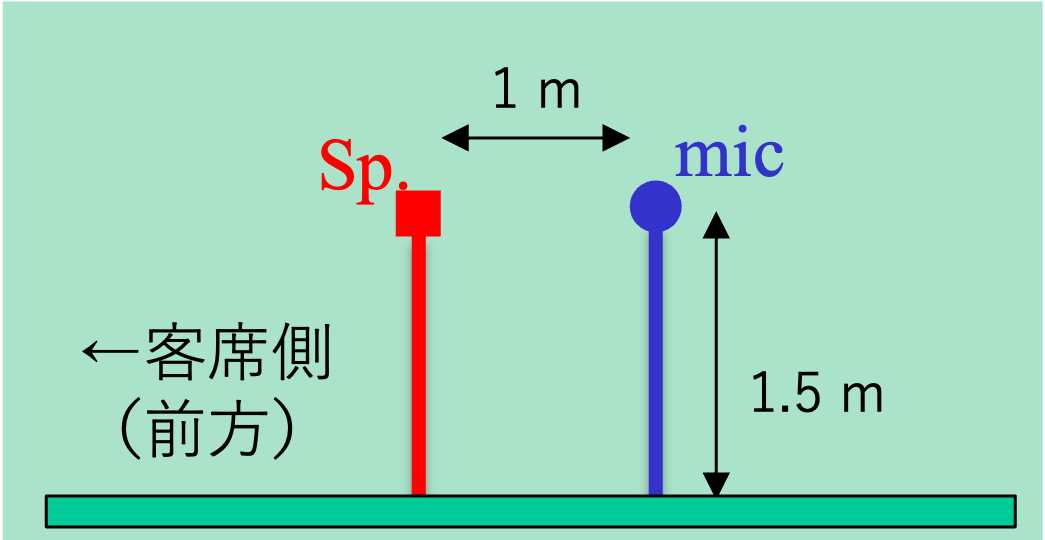
\includegraphics[width=6.5cm,clip]{images/howToMeasureST.png}
  \caption{STのインパルス応答測定条件の概略図}
  \label{fig:STのIR測定条件}
\end{figure}

%=======================================================================
\newpage
\subsection*{アンビソニックマイクを用いた測定システム}
本研究における受音系のマイクとして、図\ref{fig:アンビソニックマイク}に示す商用のアンビソニックマイク(Ambeo VR Mic, Sennheiser)を用いた。アンビソニックマイクは4つのカージオイド特性のマイクを正四面体の頂点方向に配置したものであり、測定後の簡単な信号処理により、全指向性マイクで測定した信号および任意の方向にカージオイド特性のマイクを向けて測定した信号と等価な信号を得ることができる\cite{西村竜一2014}。本研究で用いたアンビソニックマイクの方向に関する定義を図\ref{fig:方向の定義}に示す。

\begin{figure}[H]
  \begin{minipage}[b]{.33\textwidth}
      \centering
      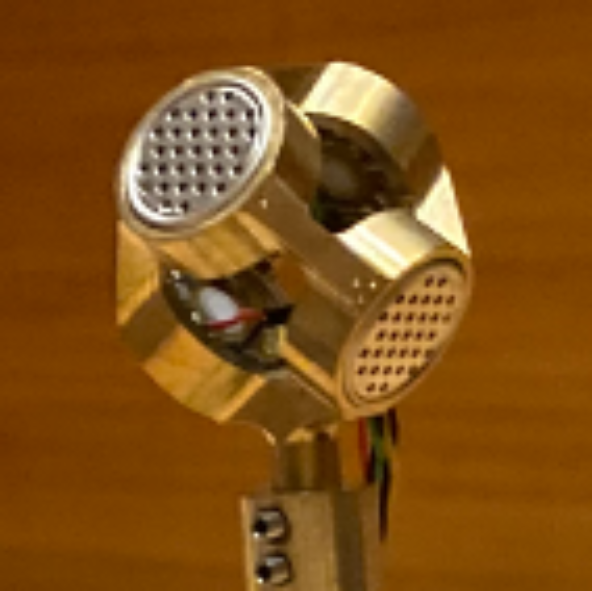
\includegraphics[width=.8\linewidth]{images/ambisonicMic.png}
      \caption{アンビソニックマイク}
      \label{fig:アンビソニックマイク}
  \end{minipage}%
  \begin{minipage}[b]{.66\textwidth}
      \centering
      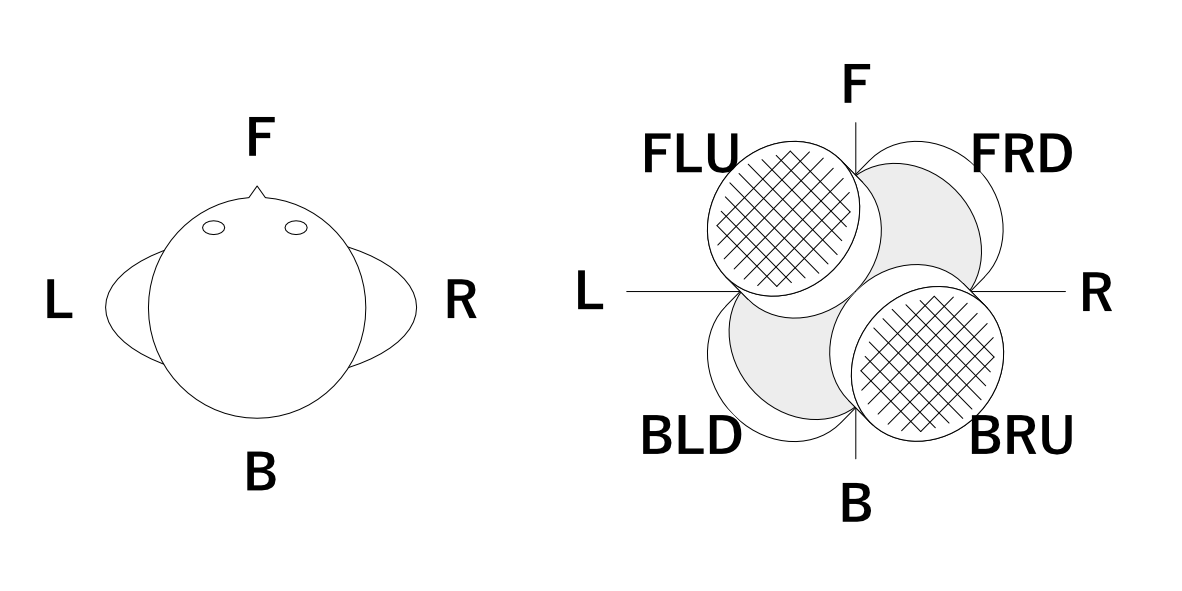
\includegraphics[width=.8\linewidth]{images/ambisonicMicDirectionDef.png}
      \caption{本研究における方向の定義}
      \label{fig:方向の定義}
  \end{minipage}
\end{figure}

方向別インパルス応答を得る手順は次の通りである。まず、Aフォーマットと呼ばれる正四面体の頂点方向の信号から式(\ref{ambisonicAtoB})により全指向性の信号と互いに直交する3つの双指向性の信号からなるBフォーマットと呼ばれる信号を得る。続いて、式(\ref{ambisonicBtoDir})によりBフォーマットの信号から直交6方向の方向別インパルス応答を計算する。

ここで、$p_(t)$は全指向性マイクで測定したインパルス応答と等価な信号、$p_{\mathrm{FB}}(t)$、$p_{\mathrm{LR}}(t)$、$p_{\mathrm{UD}}(t)$は前後、左右、上下の双指向性マイクで収録したインパルス応答と等価な信号を表し、$p_{\mathrm{FLU}}$、$p_{\mathrm{FRD}}$、$p_{\mathrm{BLD}}$、$p_{\mathrm{BRU}}$はアンビソニックマイクのうち前方左上方(Front Left Up)、前方右下方(Front Right Down)、後方左下方(Back Left Down)、後方右上方(Back Right Up)の信号を表す。
\begin{equation}
  \label{ambisonicAtoB}
  \begin{alignedat}{4}
    p_(t) &= \frac{1}{2} (p_{\mathrm{FLU}} + p_{\mathrm{FRD}} + p_{\mathrm{BLD}} + p_{\mathrm{BRU}})
    \\
    p_{\mathrm{FB}}(t) &= \frac{\sqrt{3}}{2} (p_{\mathrm{FLU}} + p_{\mathrm{FRD}} - p_{\mathrm{BLD}} - p_{\mathrm{BRU}})
    \\
    p_{\mathrm{LR}}(t) &= \frac{\sqrt{3}}{2} (p_{\mathrm{FLU}} - p_{\mathrm{FRD}} + p_{\mathrm{BLD}} - p_{\mathrm{BRU}})
    \\
    p_{\mathrm{UD}}(t) &= \frac{\sqrt{3}}{2} (p_{\mathrm{FLU}} - p_{\mathrm{FRD}} - p_{\mathrm{BLD}} + p_{\mathrm{BRU}})
    \\
  \end{alignedat}
\end{equation}
\begin{equation}
  \label{ambisonicBtoDir}
  \begin{alignedat}{6}
    p_{\mathrm{F}}(t) &= \frac{1}{2} (p(t) + p_{\mathrm{FB}}(t))
    \\
    p_{\mathrm{B}}(t) &= \frac{1}{2} (p(t) - p_{\mathrm{FB}}(t))
    \\
    p_{\mathrm{L}}(t) &= \frac{1}{2} (p(t) + p_{\mathrm{LR}}(t))
    \\
    p_{\mathrm{R}}(t) &= \frac{1}{2} (p(t) - p_{\mathrm{LR}}(t))
    \\
    p_{\mathrm{U}}(t) &= \frac{1}{2} (p(t) + p_{\mathrm{UD}}(t))
    \\
    p_{\mathrm{D}}(t) &= \frac{1}{2} (p(t) - p_{\mathrm{UD}}(t)) \\
  \end{alignedat}
\end{equation}

%=======================================================================
\section{方向別STの実測}

\subsection*{測定方法および測定結果}
前節で提案した方向別STについて、室形状・空間規模の異なる複数のホールの多数点で方向別
実測を行い、現実のホールステージにおける反射音到来方向特性を把握する。音源には図\ref{fig:対向スピーカー}に示す無指向性の対向スピーカー、マイクロホンには図\ref{fig:アンビソニックマイク}に示す商用の1次アンビソニックマイク(Ambeo VR Mic, Sennheiser)を使用した。

音響測定を実施した各ホールの諸元を\ref{table:全ホールの諸元}に示す。ホールAからFは舞台を反射板形式とした多目的ホール、ホールGはアリーナ型のコンサートホールである。なお、ホールBは天井反射板が無い舞台となっている。また、測定を実施した各ホールの外観を\ref{fig:全ホールの写真}に示す。測定点は各ホールの舞台の上手側半面に$\SI{2}{\m}$間隔のグリッド上に配置した。\ref{fig:各ホールの測定位置}に各ホールにおける測定点の音源位置を示す。全ての測定点において音源を客席側、マイクを舞台奥側に配置している。

各ホールのすべての測定点における測定結果を図\ref{fig:ホールA 方向別ST}から図\ref{fig:ホールG 方向別ST}に示す。測定位置によって$\SI{10}{\ms}$から$\SI{20}{\ms}$にも反射音のエネルギーが到来し、これも踏まえた考察を行うため、前節で提案した$\mathrm{ST_{Early,dir}}$および$\mathrm{ST_{Late,dir}}$に加え、$\SI{10}{\ms}$から$\SI{100}{\ms}$の時間窓で反射音を評価した結果についても合わせて示した。
\\

\begin{figure}[H]
  \centering
  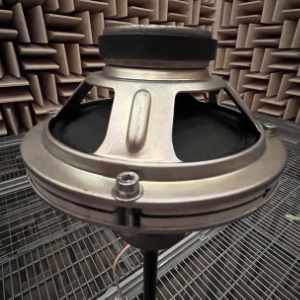
\includegraphics[width=.3\linewidth]{images/measuredHalls/opposedSpeaker.jpg}
  \caption{対向スピーカー}
  \label{fig:対向スピーカー}
\end{figure}

\begin{table}[H]
  \centering
  \caption{測定を実施したホールの諸元}
  \label{table:全ホールの諸元}
  \begin{tabular}{cccccccc} \hline \hline
    ホール &
    \begin{tabular}{c}
      座席数\\
      (席)
    \end{tabular}& 
    \begin{tabular}{c}
      $\mathrm{T_{30}}$(s) 500-\\
      1kHz平均
    \end{tabular}&
    \begin{tabular}{c}
      室容積\\
      ($\mathrm{m^{3}}$)
    \end{tabular}&
    \begin{tabular}{c}
      表面積\\
      ($\mathrm{m^{2}}$) 
    \end{tabular}&
    \begin{tabular}{c}
      舞台間口\\
      (m)
    \end{tabular}&
    \begin{tabular}{c}
      舞台奥行\\
      (m)
    \end{tabular}&
    \begin{tabular}{c}
      舞台高さ\\(m)
    \end{tabular} \\ \hline
    A & 421 & 1.3 & 4420 & 2070 & 16.5 & 10.5 & 8 \\
    B & 500 & 1.4 & 5680 & 2740 & 15.5 & 9 & 7.4 \\
    C & 698 & 2.5 & 11150 & 4600 & 12 & 16.2 & 13 \\
    D & 1033 & 1.9 & 11940 & 4380 & 20 & 10 & 10 \\
    E & 1104 & 1.6 & 10225 & 3435 & 19 & 9 & 8 \\
    F & 1514 & 2.3 & 15580 & 5860 & 18.2 & 18.2 & 15 \\
    G & 1884 & 2.2 & 18610 & 6445 & 20.8 & 11.7 & - \\ \hline \hline
  \end{tabular}
\end{table}

%=======================================================================

\newpage
\begin{figure}[H]
  \centering
  \begin{minipage}[b]{.5\textwidth}
    \centering
    \includegraphics[width=.9\linewidth]{images/measuredHalls/w90h60/picture_a.jpg}
    \caption*{ホールA}
  \end{minipage}%
  \begin{minipage}[b]{.5\textwidth}
    \centering
    \includegraphics[width=.9\linewidth]{images/measuredHalls/w90h60/picture_b.jpg}
    \caption*{ホールB}
  \end{minipage}

  \begin{minipage}[b]{.5\textwidth}
    \centering
    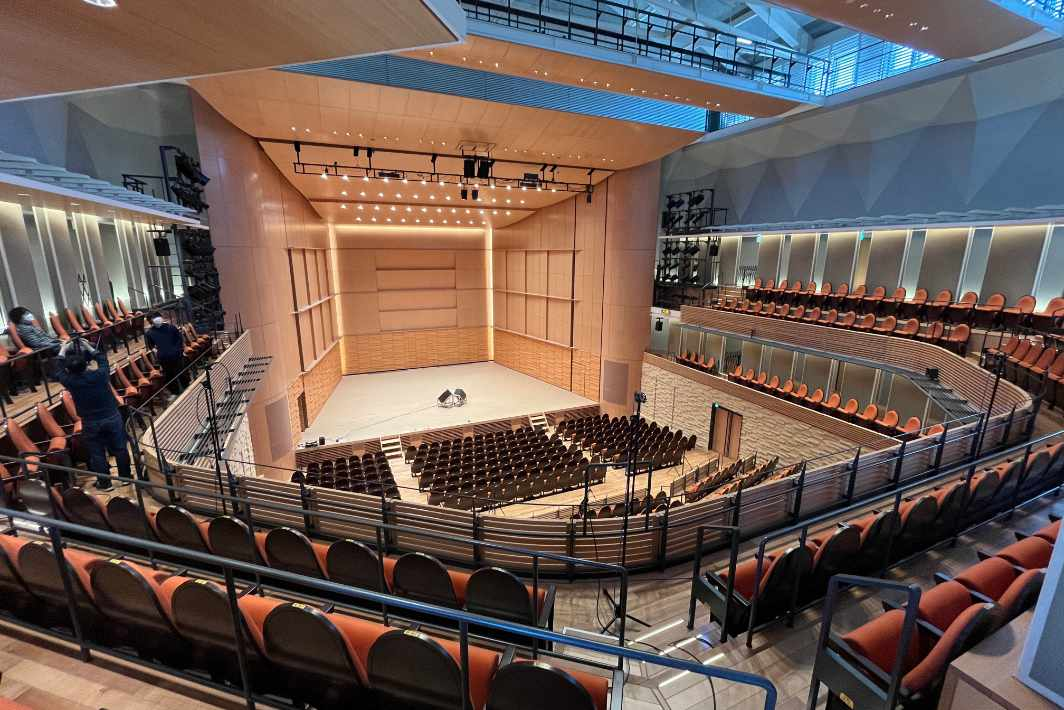
\includegraphics[width=.9\linewidth]{images/measuredHalls/w90h60/picture_c.jpg}
    \caption*{ホールC}
  \end{minipage}%
  \begin{minipage}[b]{.5\textwidth}
    \centering
    \includegraphics[width=.9\linewidth]{images/measuredHalls/w90h60/picture_d.jpg}
    \caption*{ホールD}
  \end{minipage}

  \begin{minipage}[b]{.5\textwidth}
    \centering
    \includegraphics[width=.9\linewidth]{images/measuredHalls/w90h60/picture_e.jpg}
    \caption*{ホールE}
  \end{minipage}%
  \begin{minipage}[b]{.5\textwidth}
    \centering
    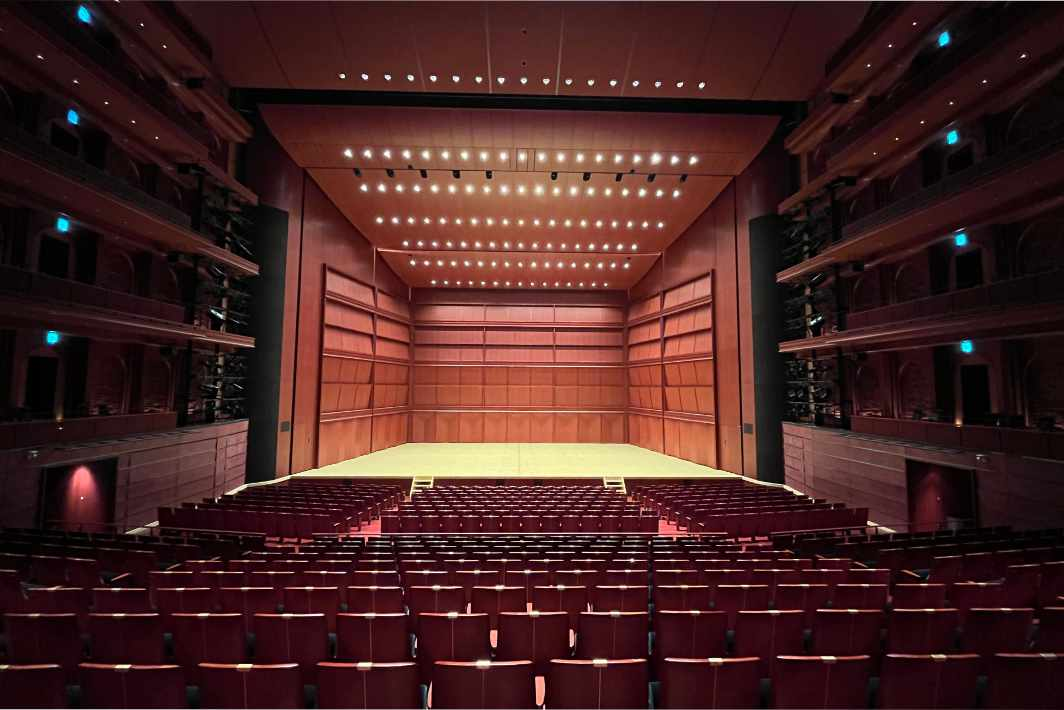
\includegraphics[width=.9\linewidth]{images/measuredHalls/w90h60/picture_f.jpg}
    \caption*{ホールF}
  \end{minipage}

  \begin{minipage}[b]{1\textwidth}
    \centering
    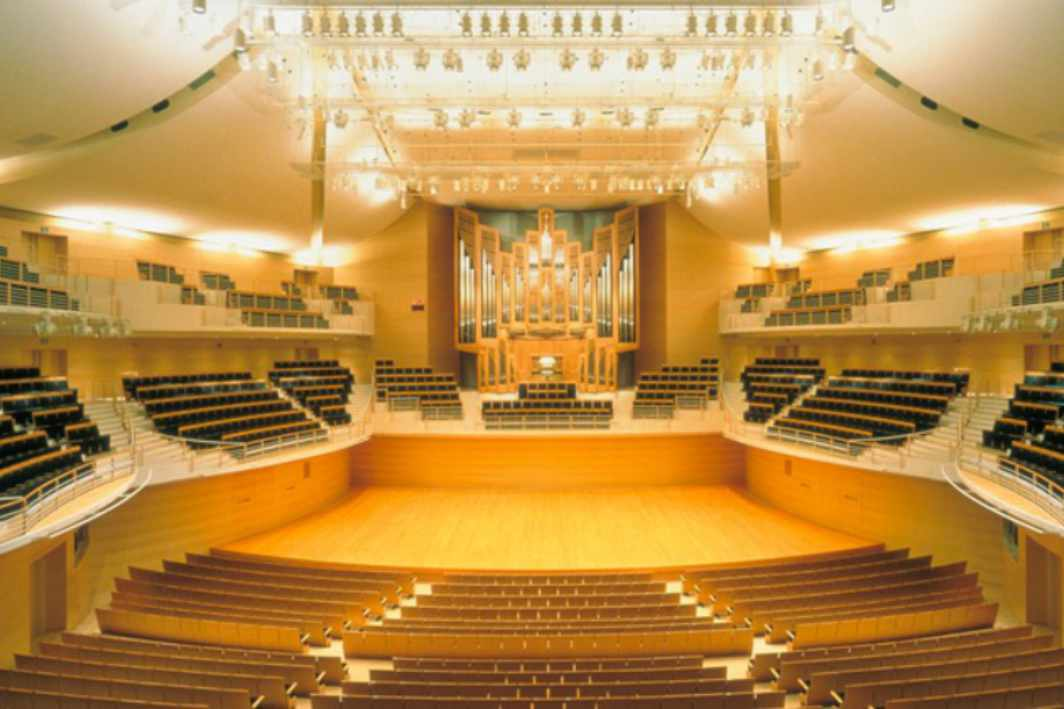
\includegraphics[width=.45\linewidth]{images/measuredHalls/w90h60/picture_g.jpg}
    \caption*{ホールG}
  \end{minipage}

  \caption{測定を実施したホールの外観}
  \label{fig:全ホールの写真}
\end{figure}

%=======================================================================

\newpage
\begin{figure}[H]
  \centering
  \begin{minipage}[b]{.5\textwidth}
    \centering
    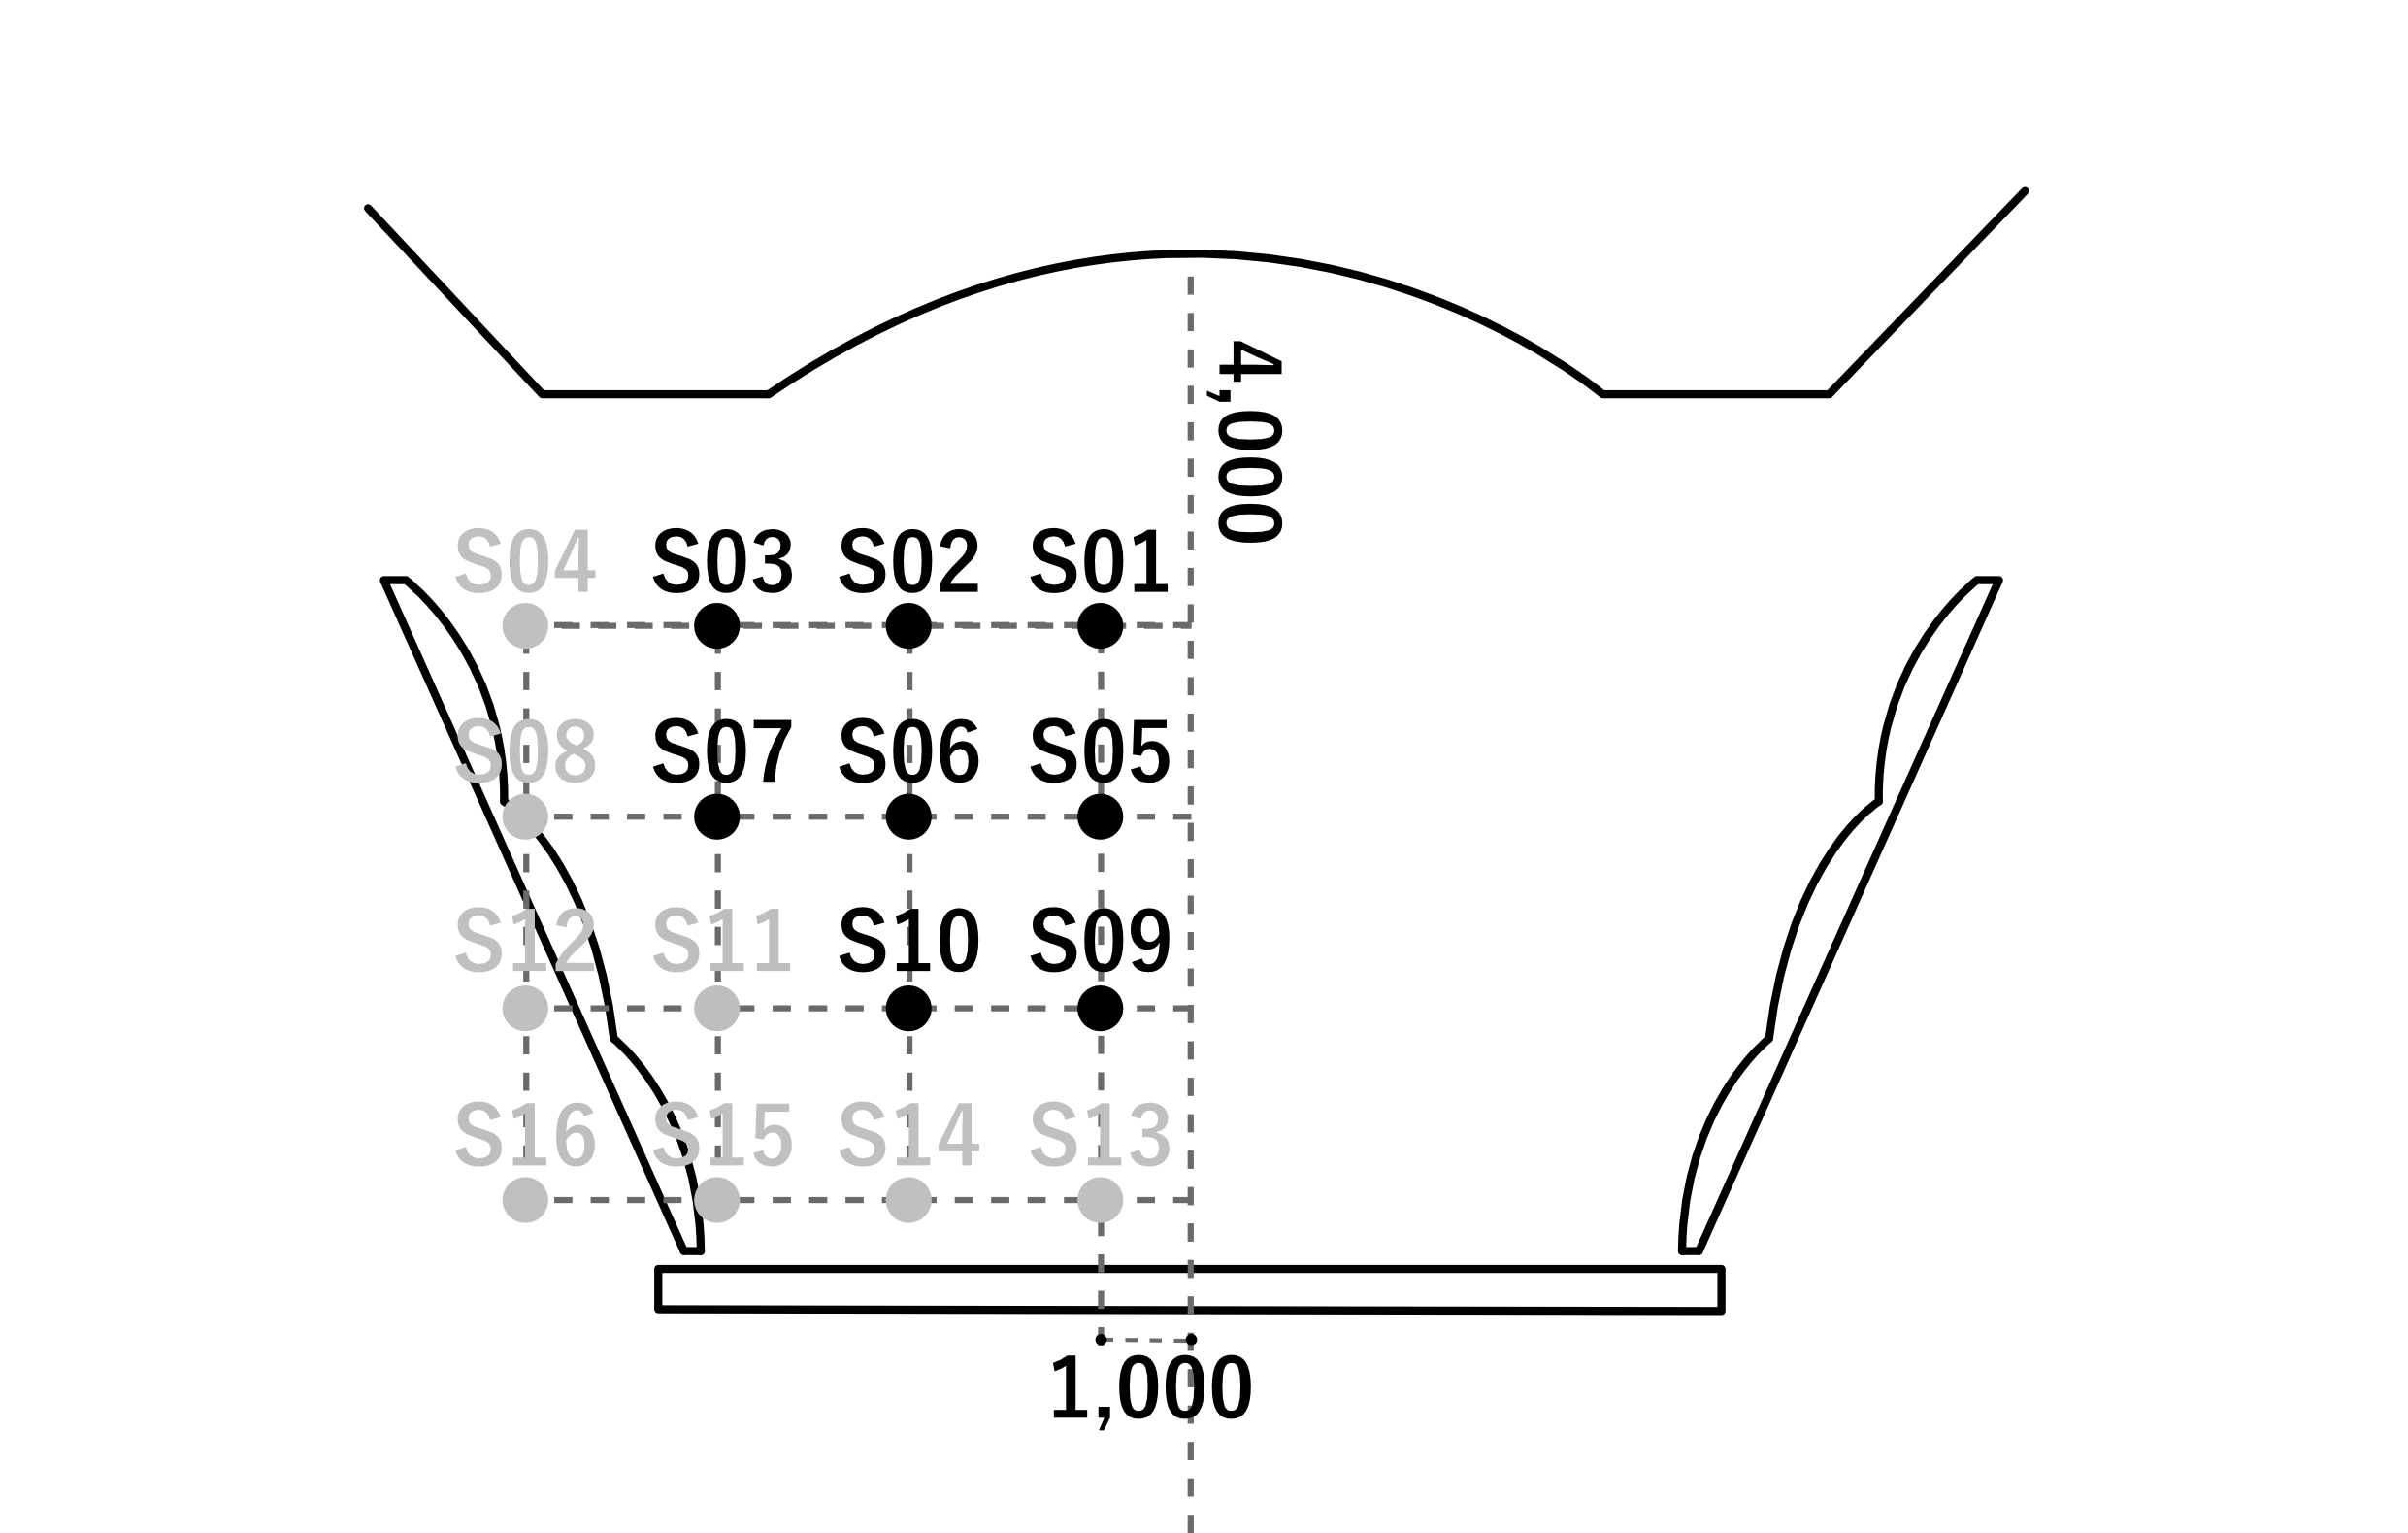
\includegraphics[width=.9\linewidth]{images/measuredHalls/flatud_hall_a.png}
    \caption*{ホールA}
  \end{minipage}%
  \begin{minipage}[b]{.5\textwidth}
    \centering
    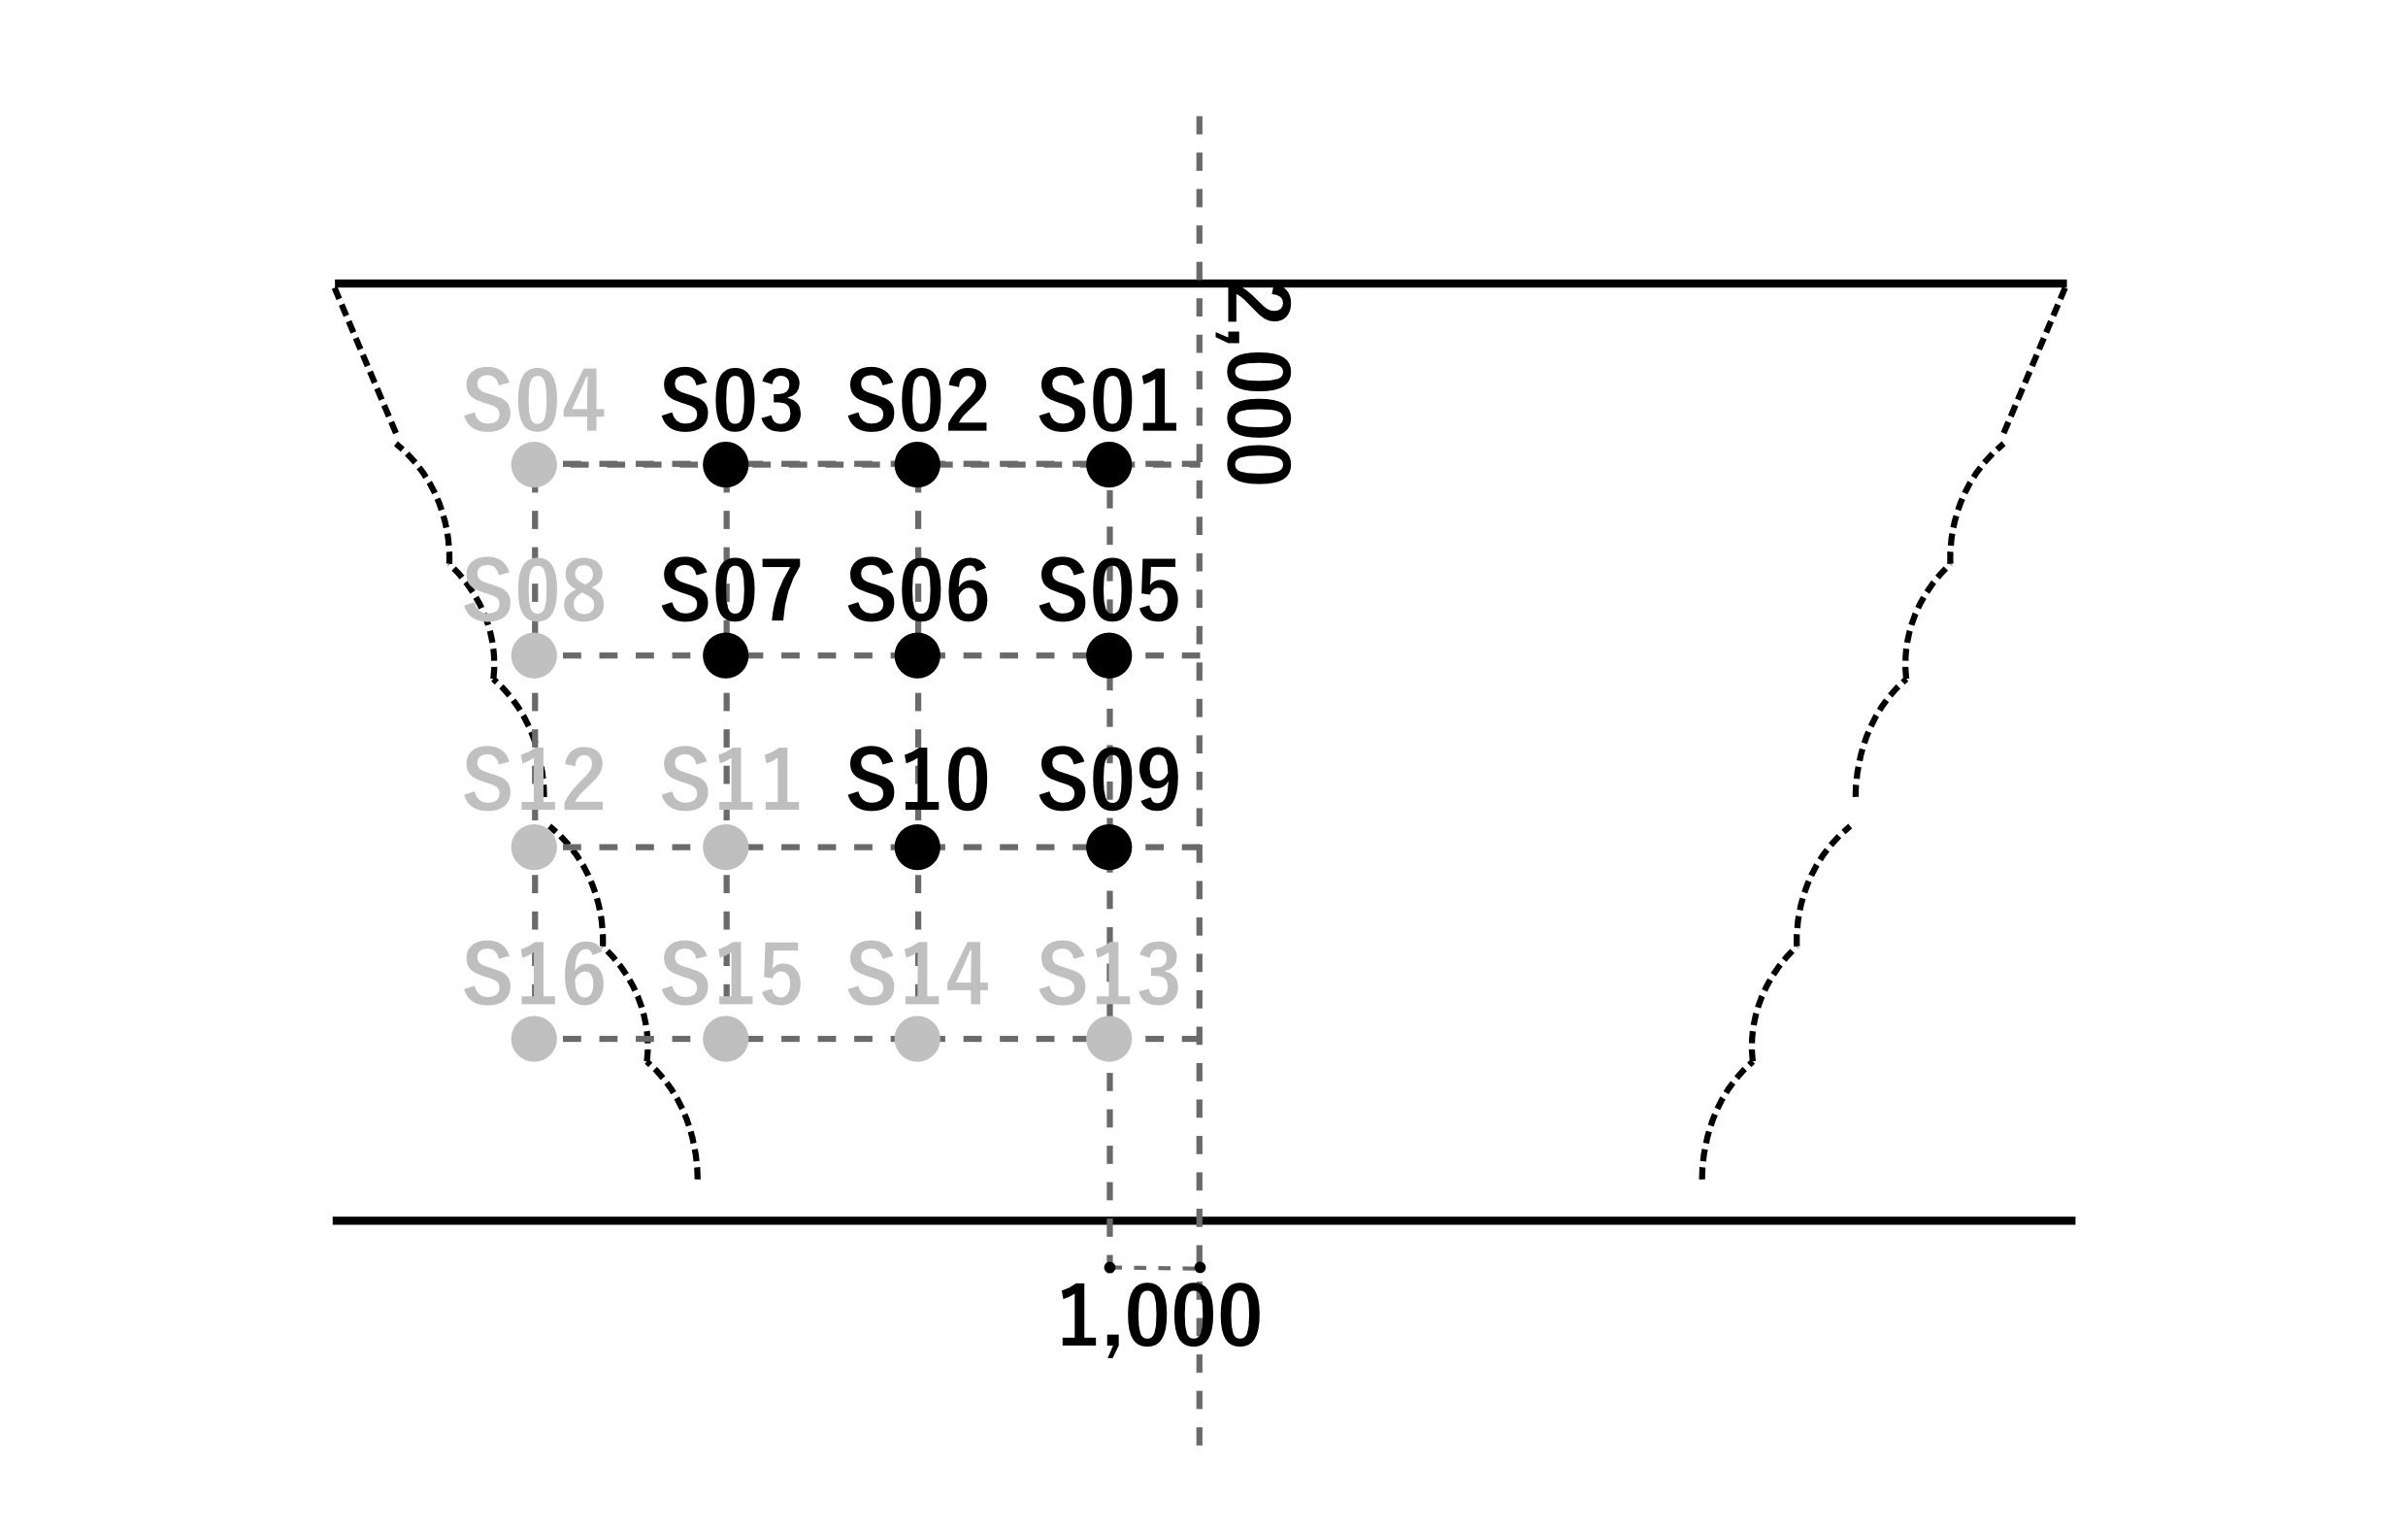
\includegraphics[width=.9\linewidth]{images/measuredHalls/flatud_hall_b.png}
    \caption*{ホールB}
  \end{minipage}

  \begin{minipage}[b]{.5\textwidth}
    \centering
    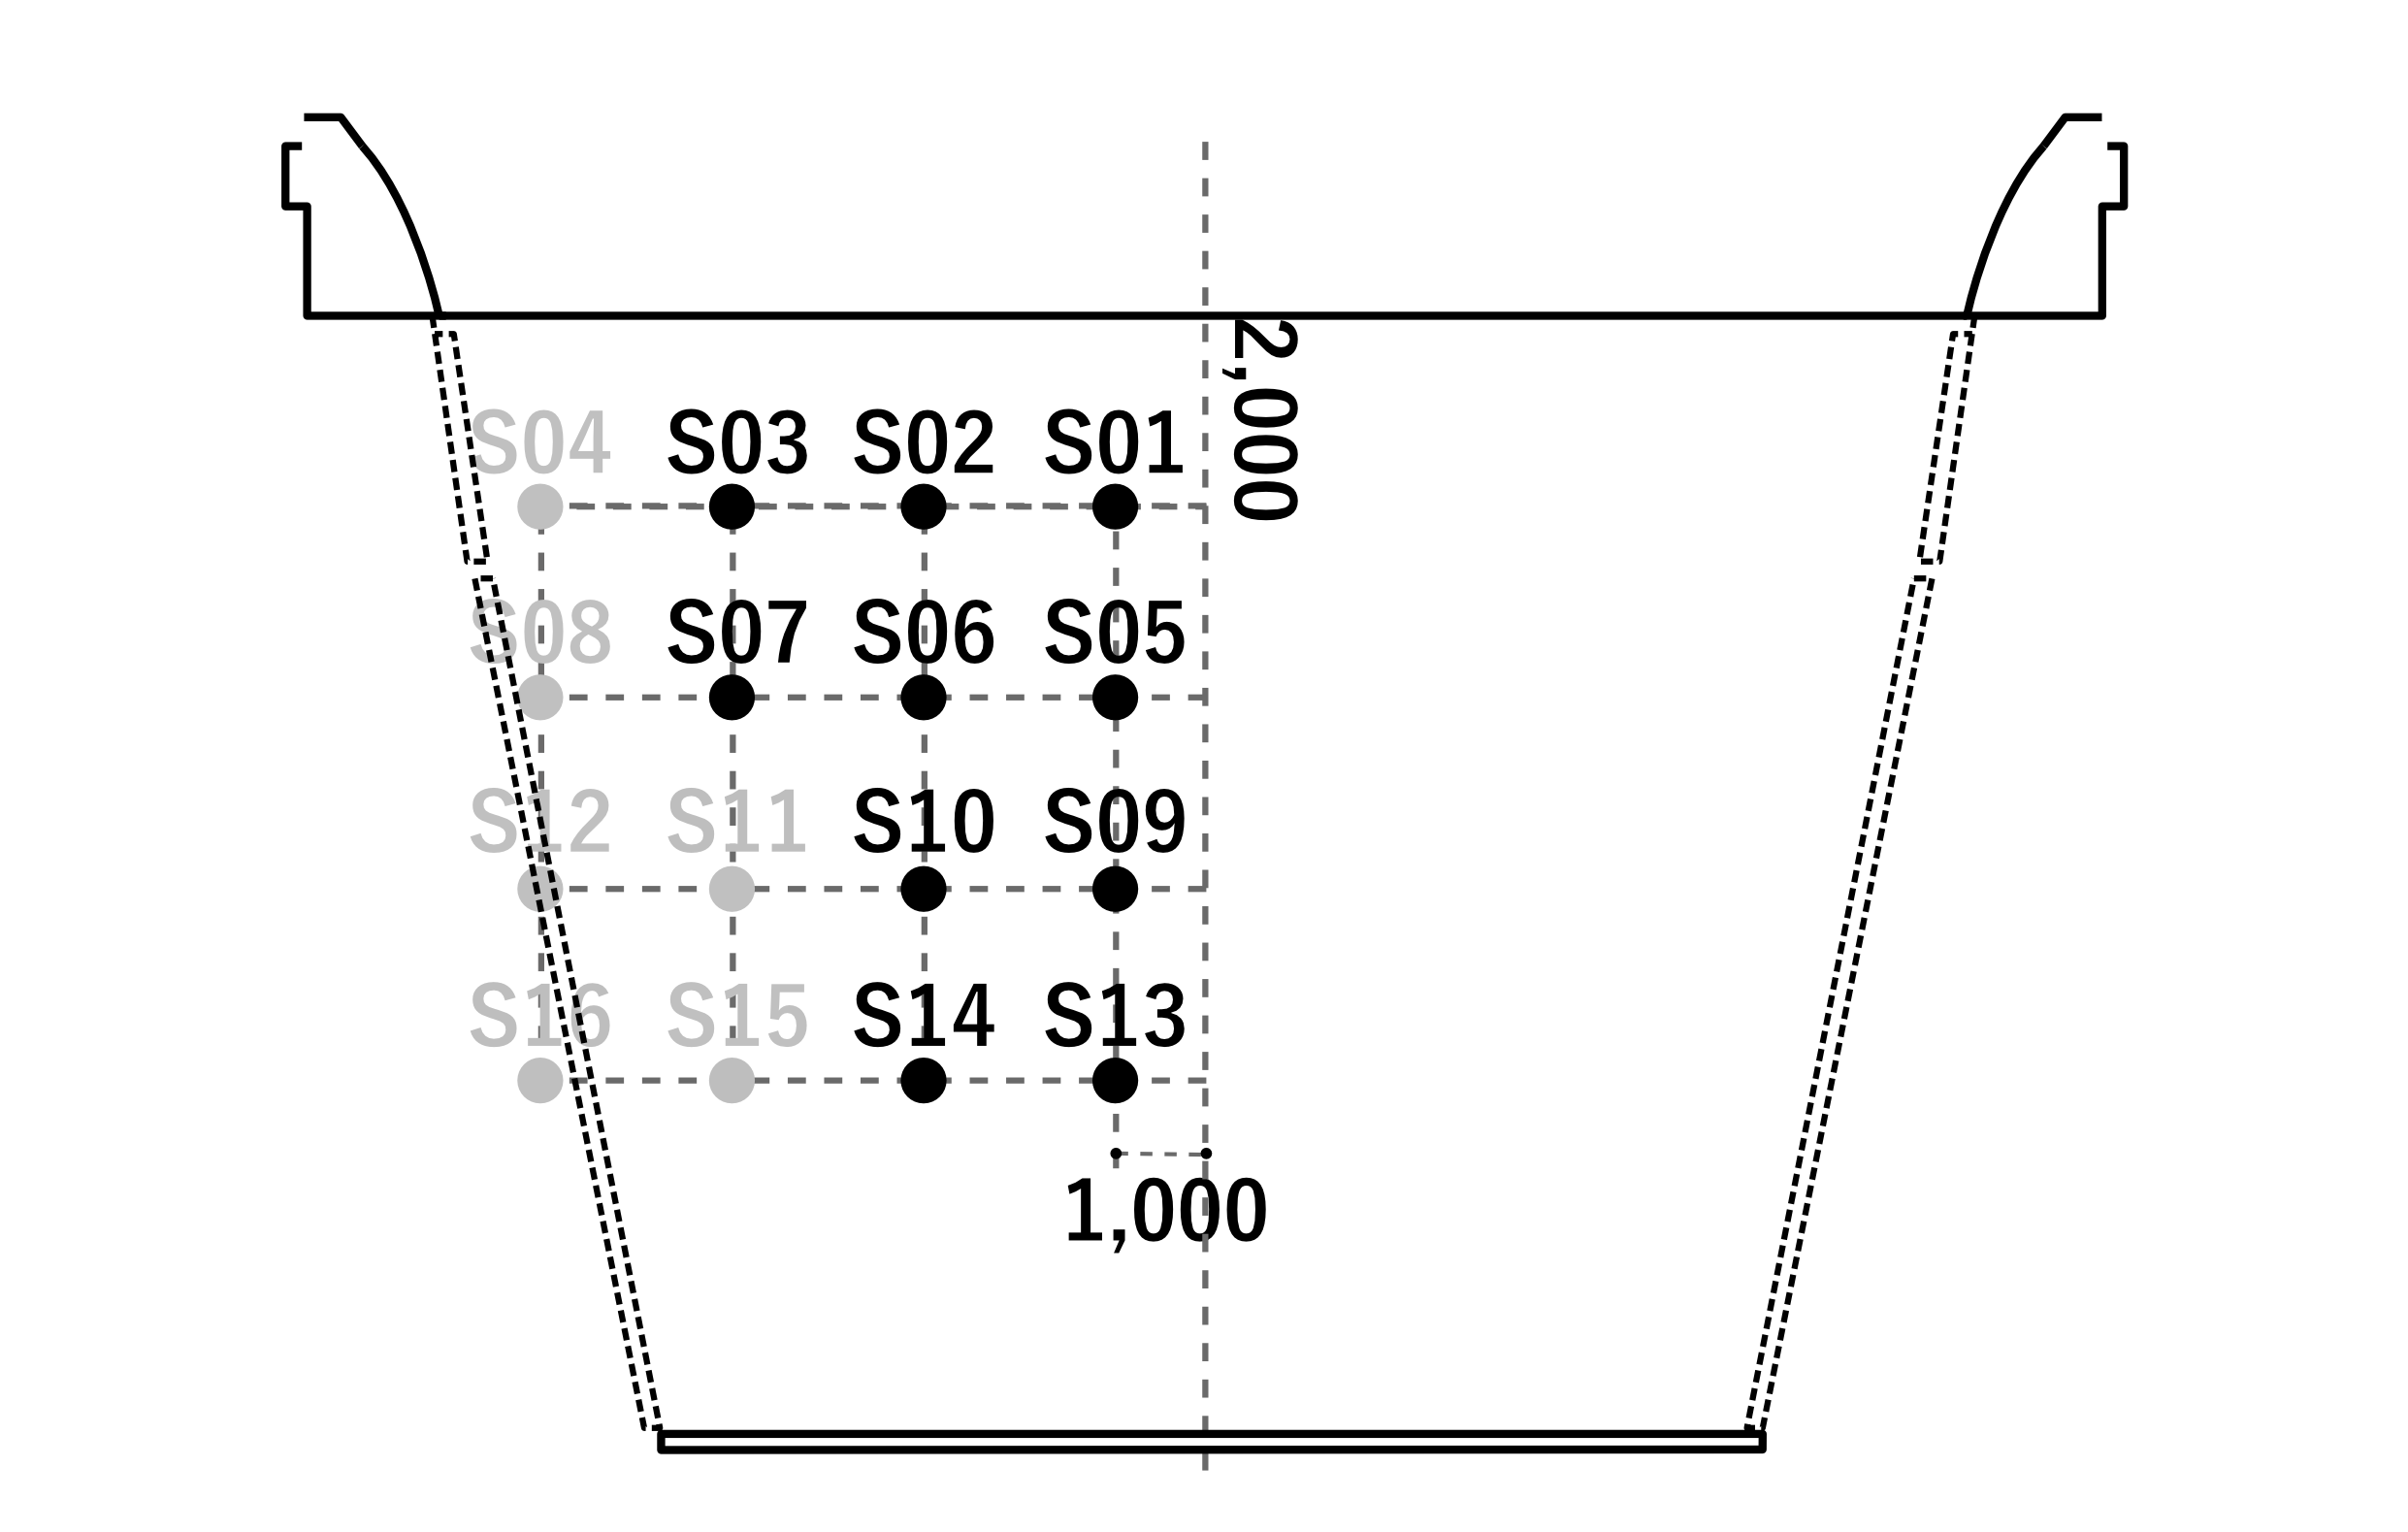
\includegraphics[width=.9\linewidth]{images/measuredHalls/flatud_hall_c.png}
    \caption*{ホールC}
  \end{minipage}%
  \begin{minipage}[b]{.5\textwidth}
    \centering
    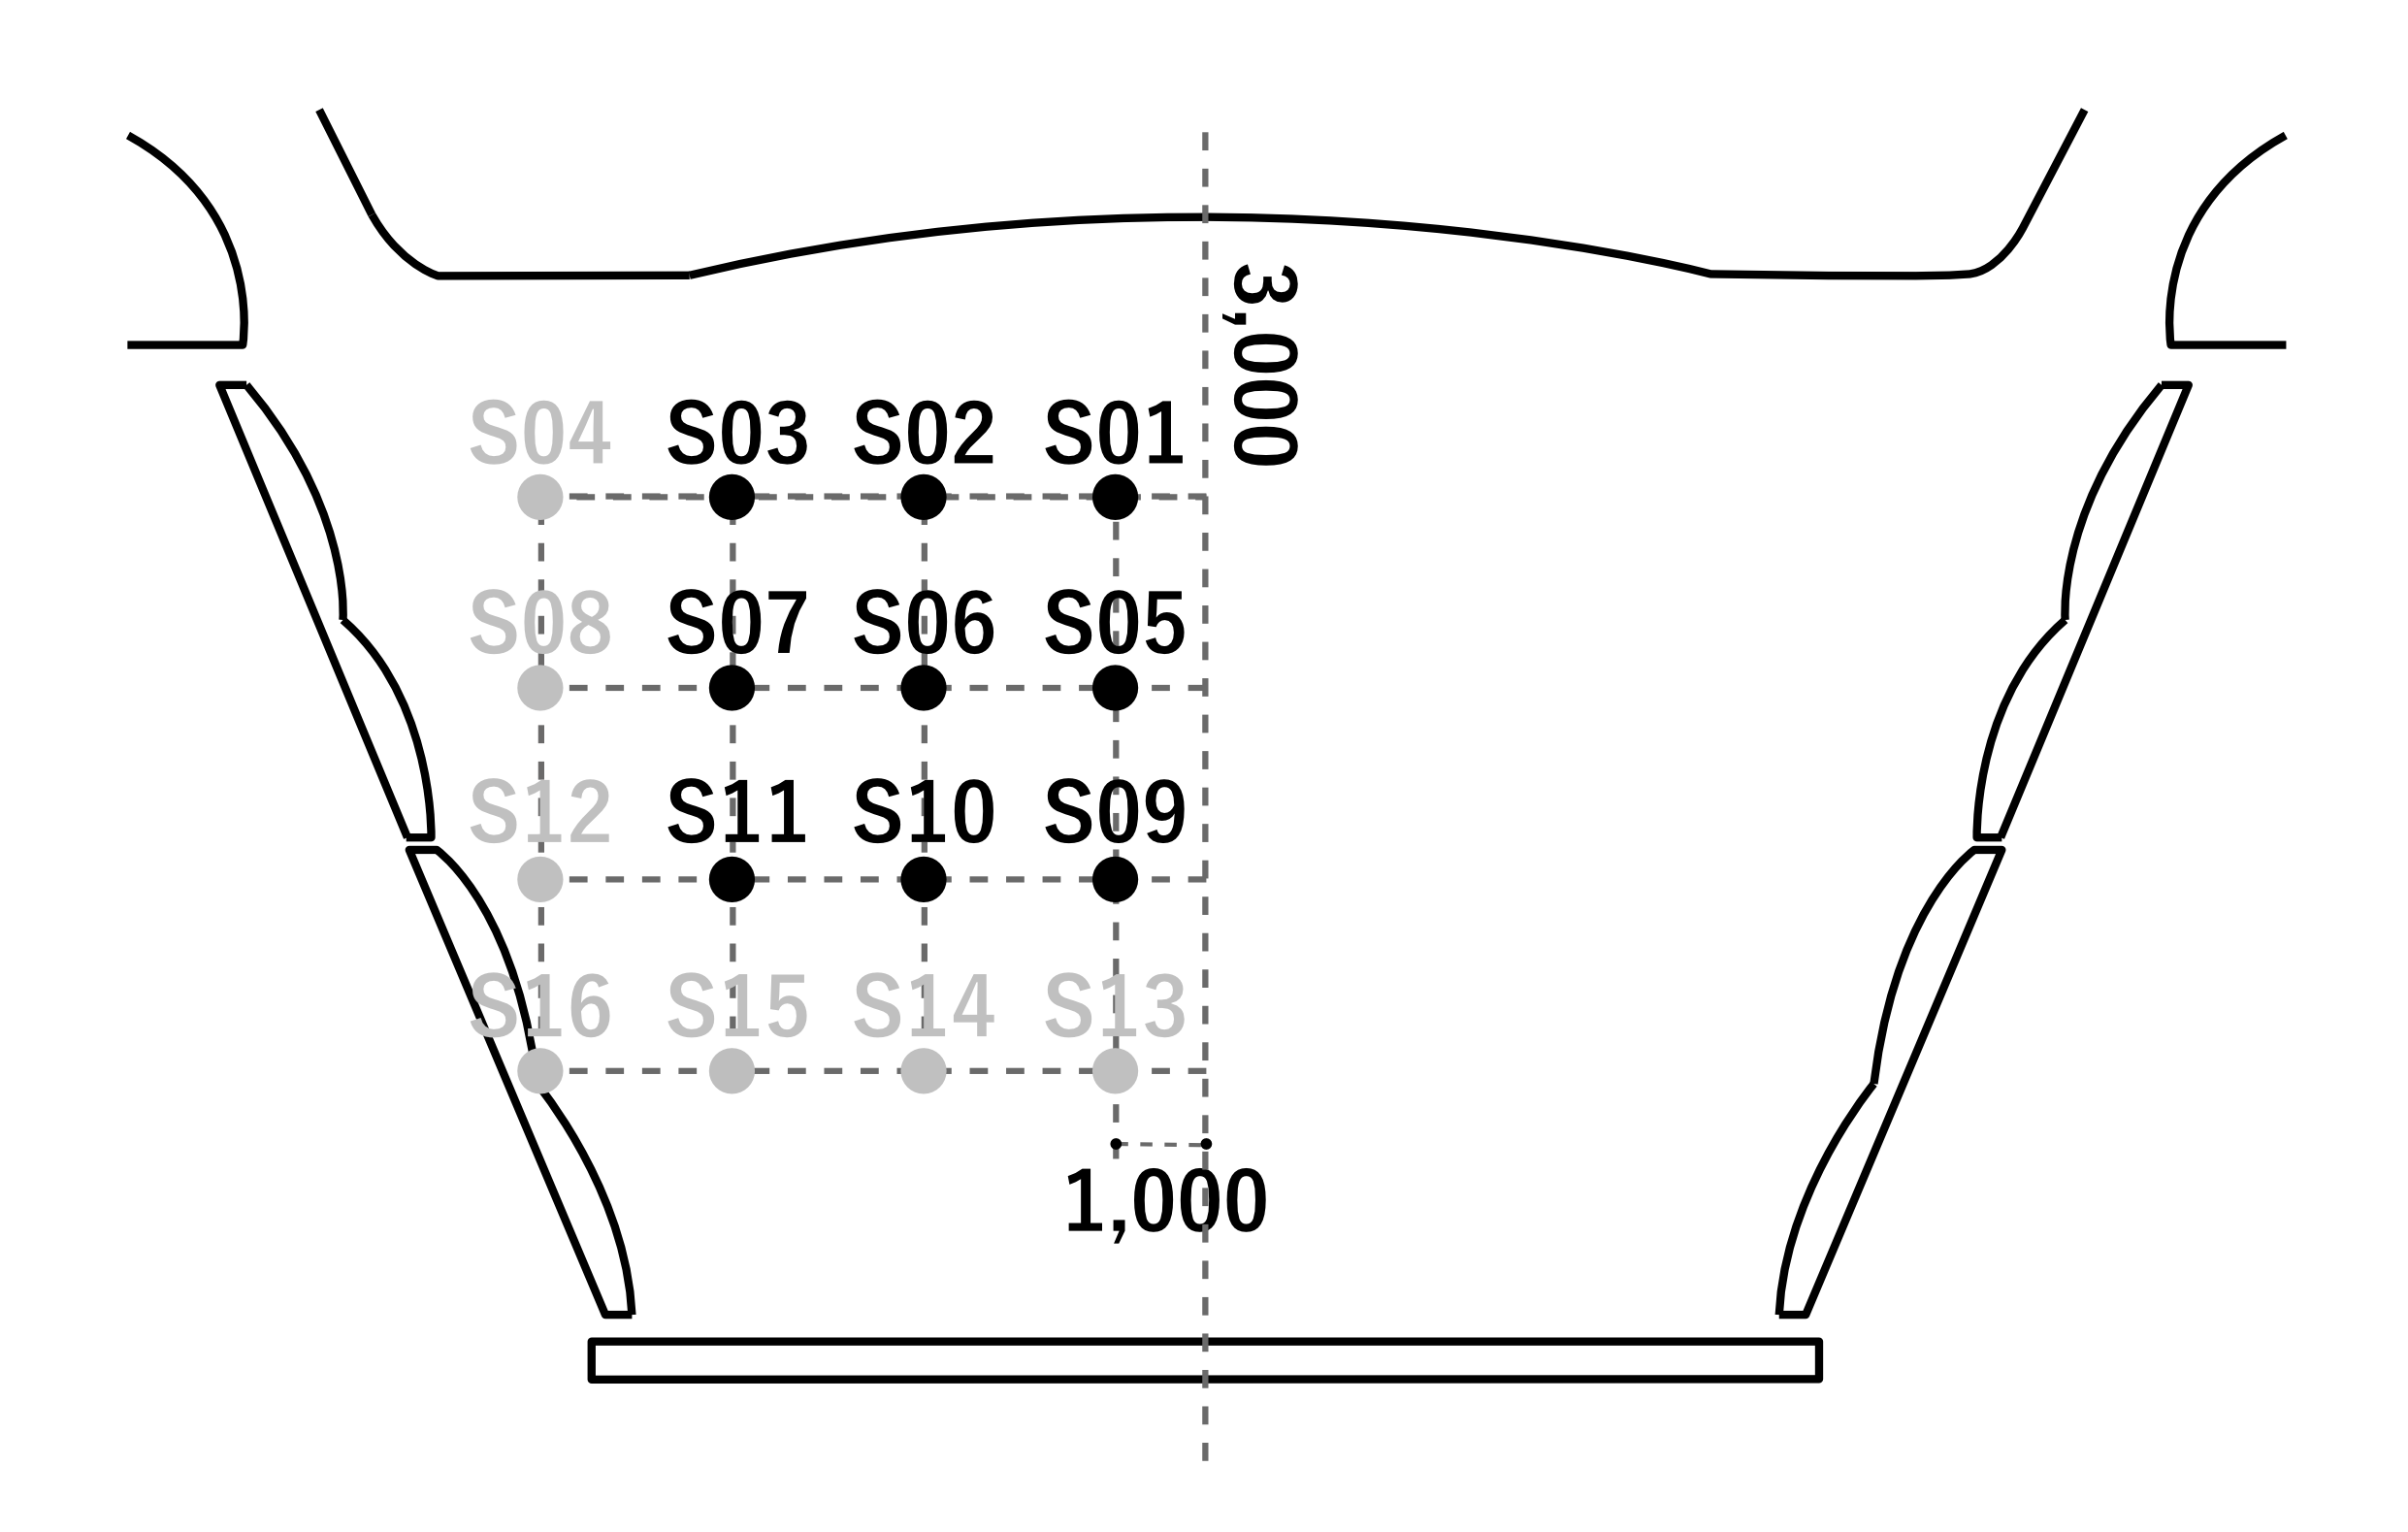
\includegraphics[width=.9\linewidth]{images/measuredHalls/flatud_hall_d.png}
    \caption*{ホールD}
  \end{minipage}

  \begin{minipage}[b]{.5\textwidth}
    \centering
    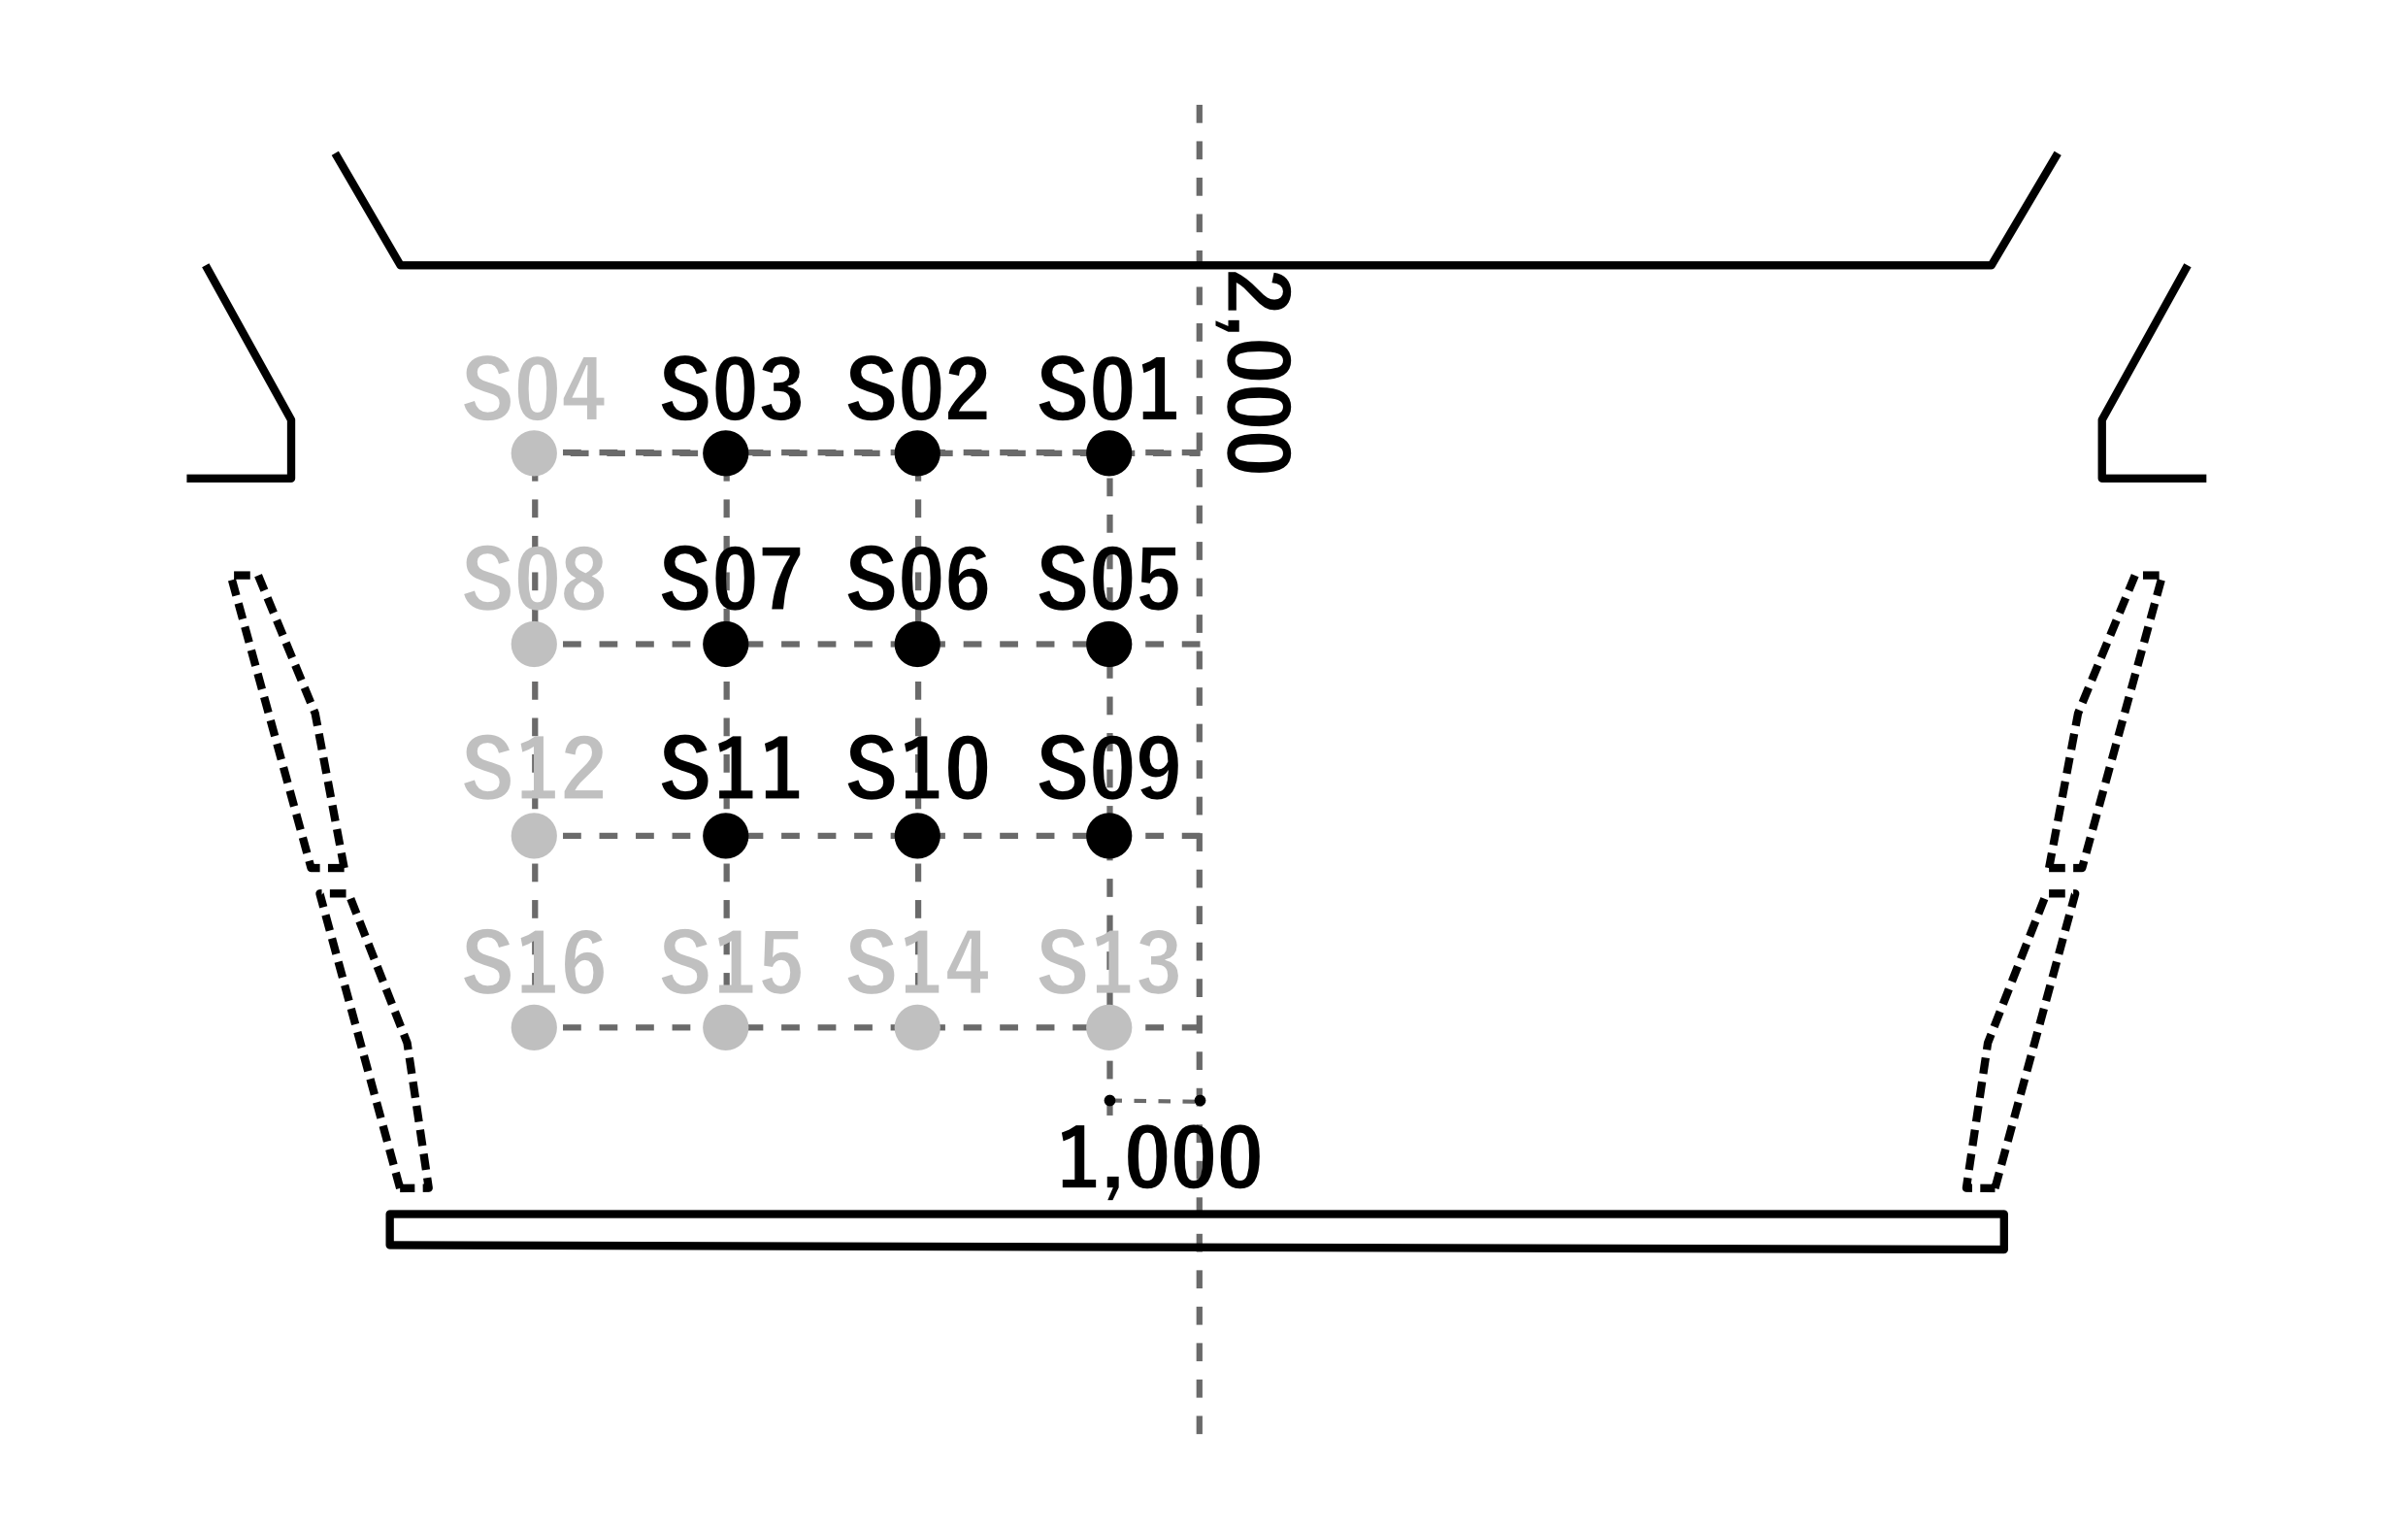
\includegraphics[width=.9\linewidth]{images/measuredHalls/flatud_hall_e.png}
    \caption*{ホールE}
  \end{minipage}%
  \begin{minipage}[b]{.5\textwidth}
    \centering
    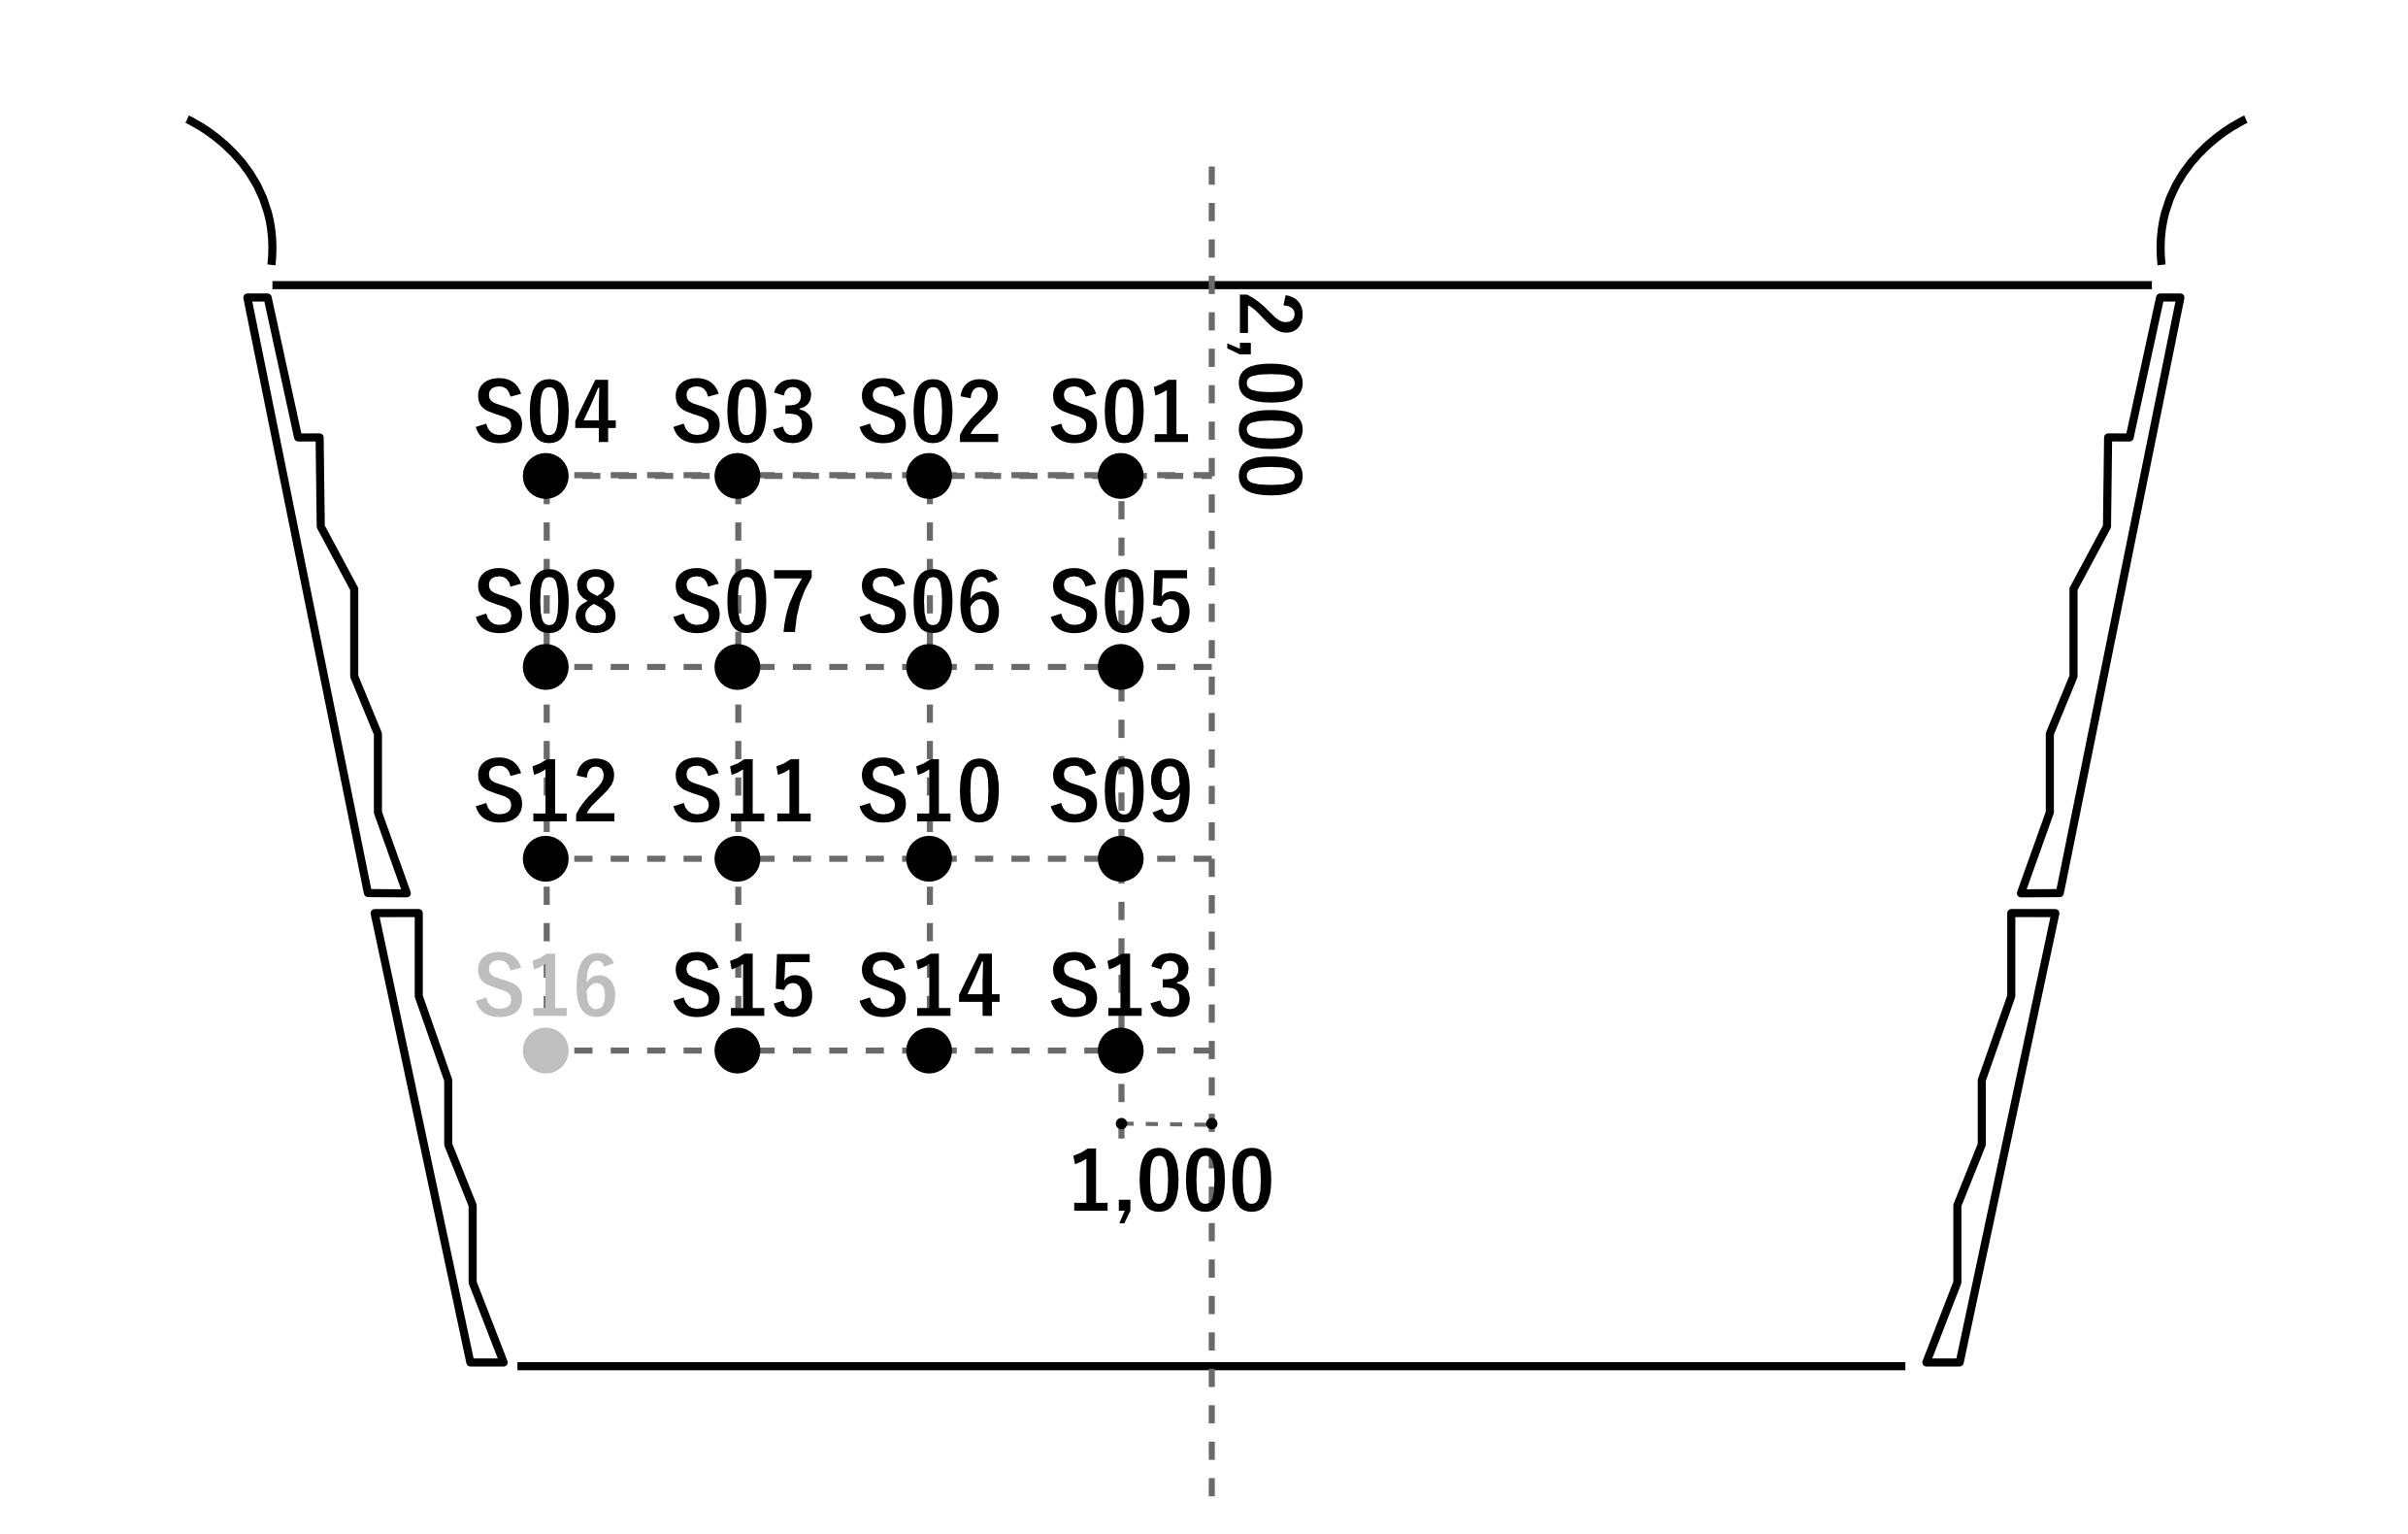
\includegraphics[width=.9\linewidth]{images/measuredHalls/flatud_hall_f.png}
    \caption*{ホールF}
  \end{minipage}

  \begin{minipage}[b]{1\textwidth}
    \centering
    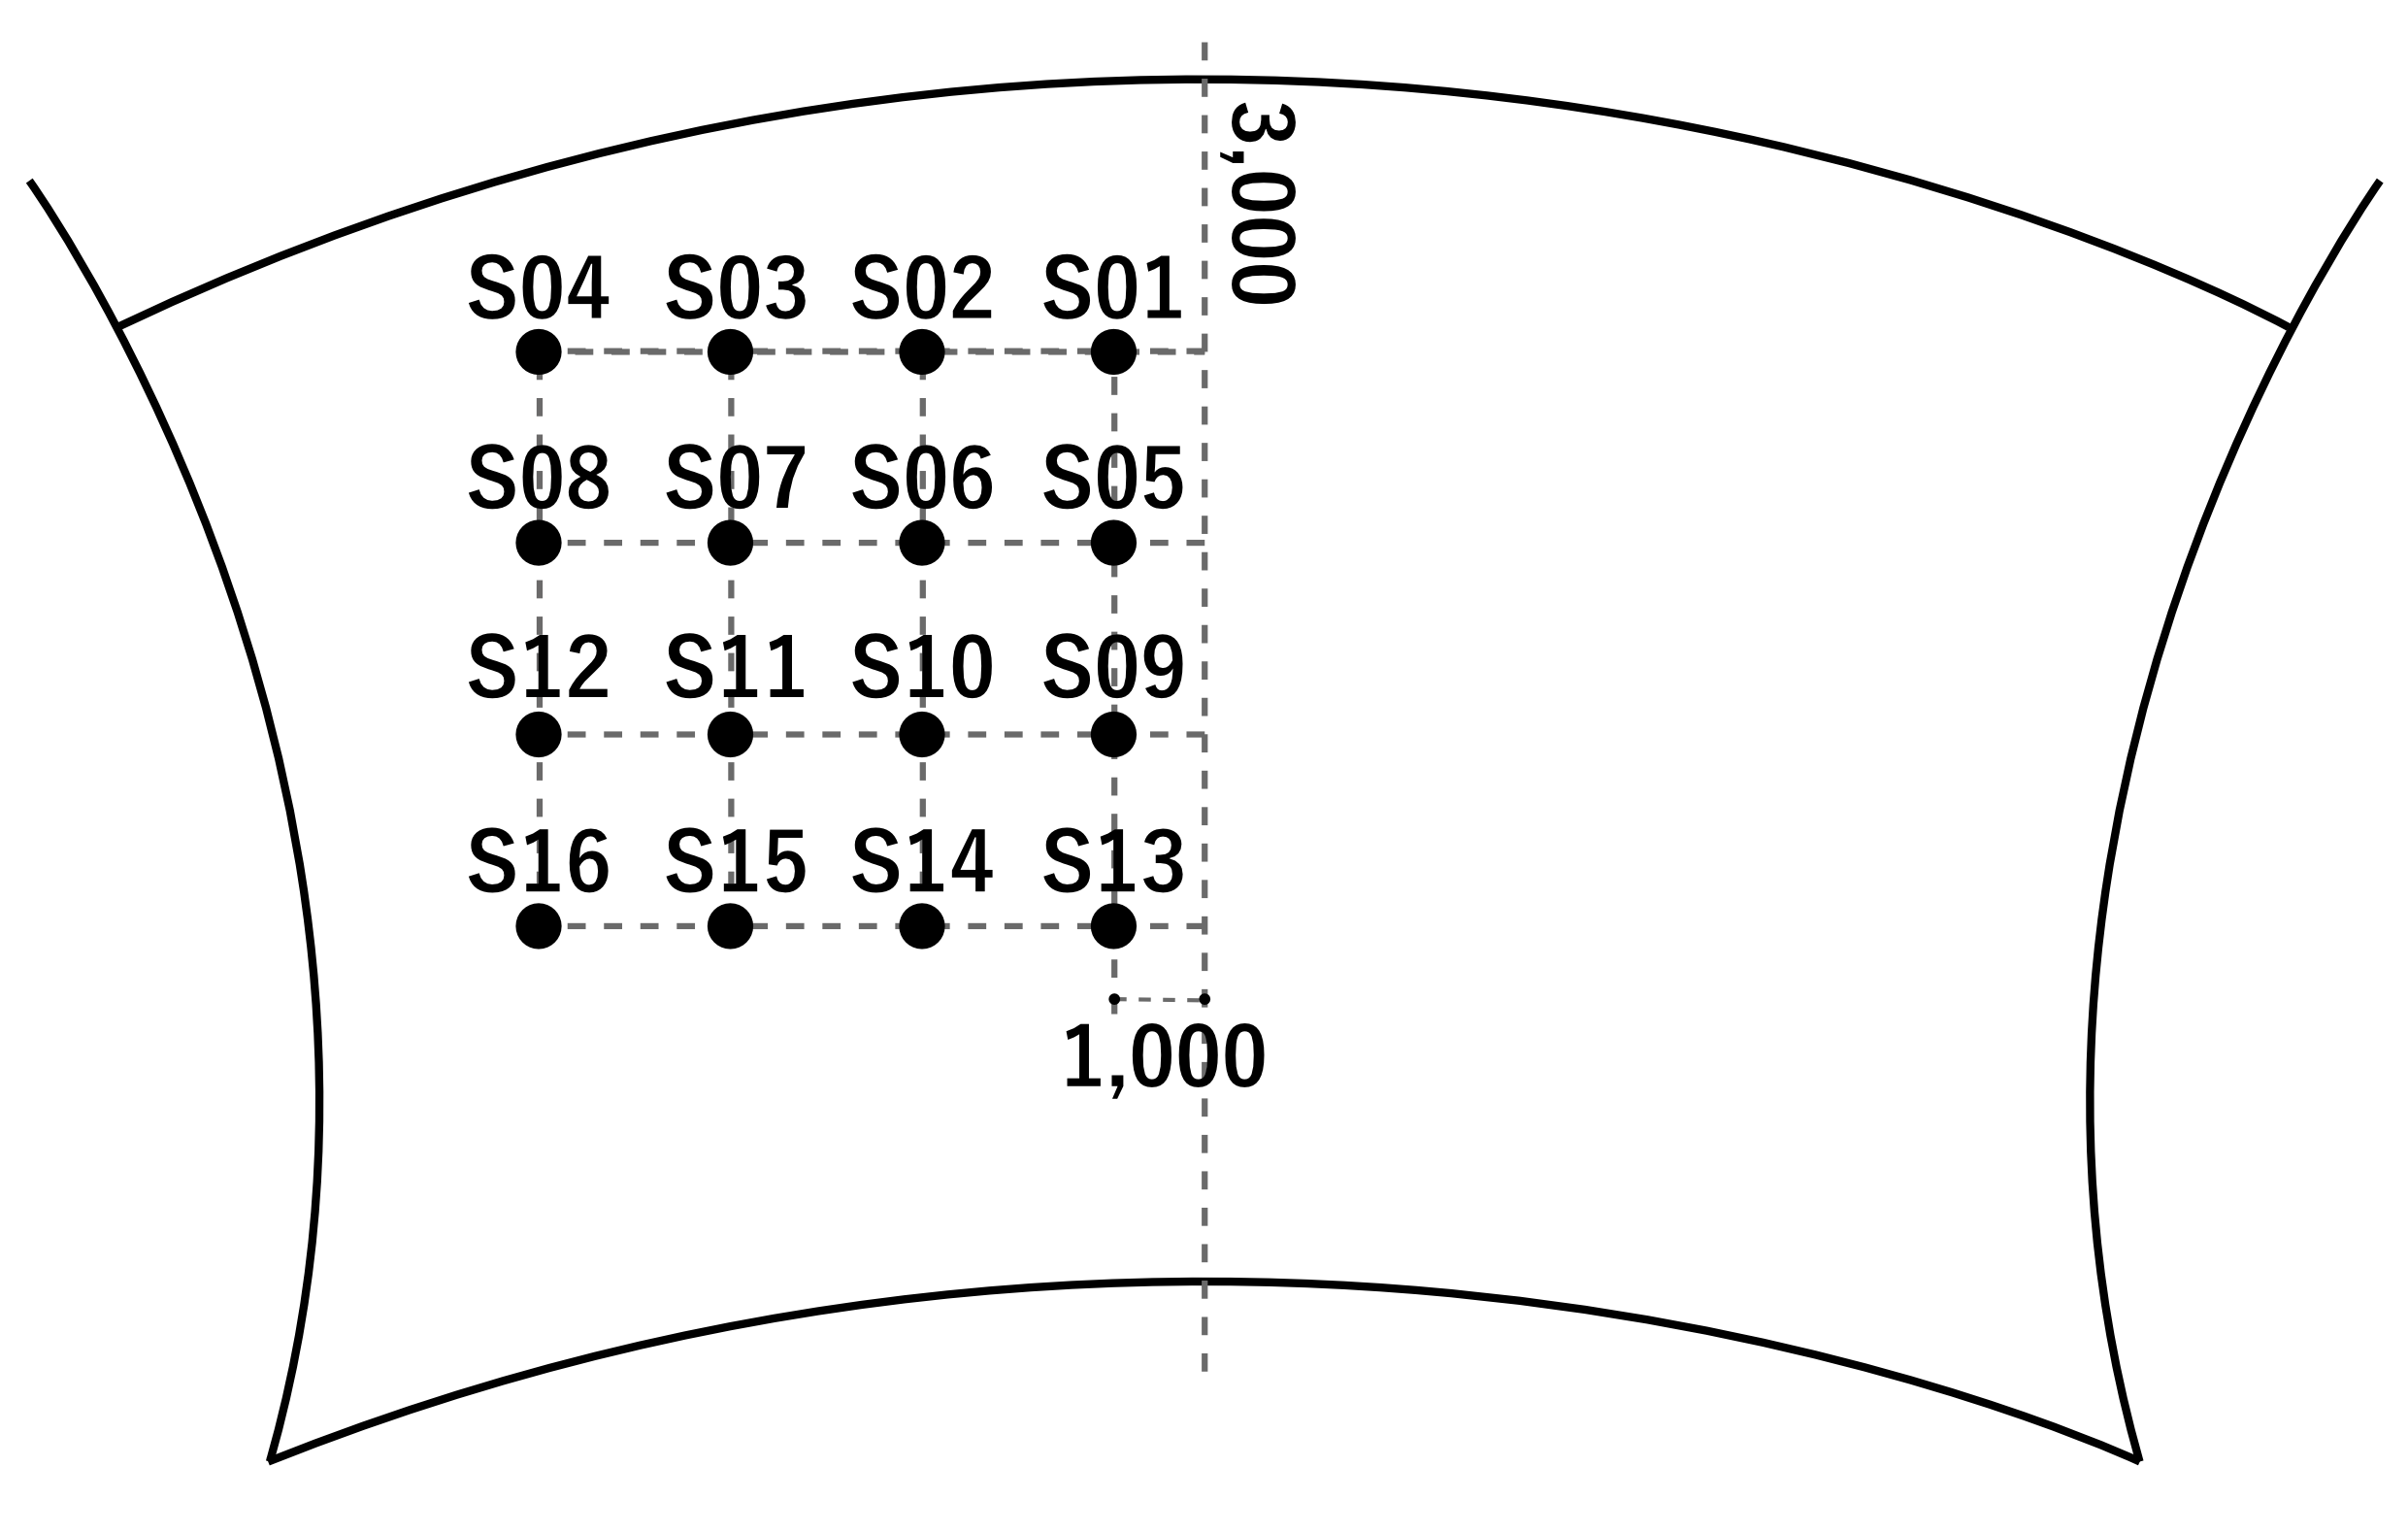
\includegraphics[width=.45\linewidth]{images/measuredHalls/flatud_hall_g.png}
    \caption*{ホールG}
  \end{minipage}

  \caption{各ホールの測定位置}
  \label{fig:各ホールの測定位置}
\end{figure}

%=======================================================================
% ホールA

\newpage
\begin{figure}[H]
  \begin{minipage}{.5\linewidth} % 右側の図
    \centering
    \includegraphics[width=.7\linewidth]{images/measuredHalls/resized/picture_a.jpg}
    \\ホールA 外観
  \end{minipage}%
  \begin{minipage}{.5\linewidth} % 右側の図
    \centering
    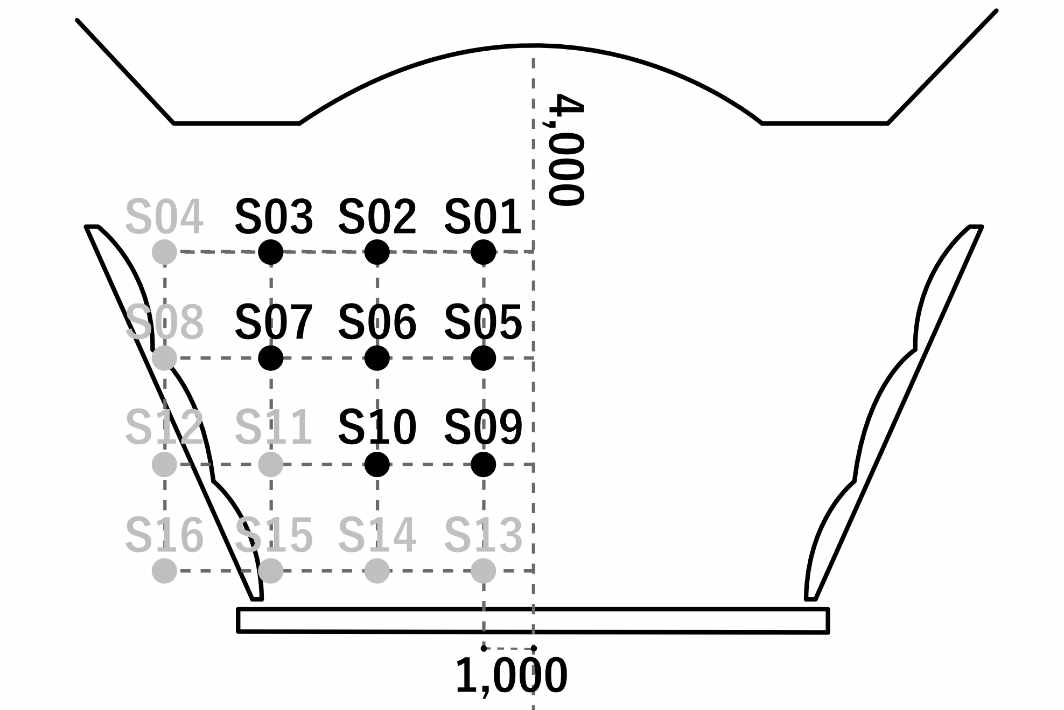
\includegraphics[width=.7\linewidth]{images/measuredHalls/resized/flat_a.jpg}
    \\ホールA 測定位置
  \end{minipage}

  \begin{minipage}{1\linewidth}
    \centering
    ホールA 諸元\\
    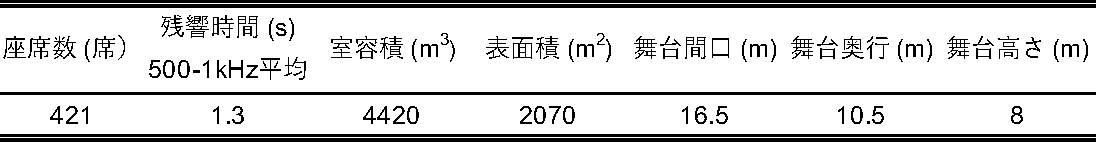
\includegraphics[width=.8\linewidth]{images/measuredHalls/informationTable/a.pdf}
  \end{minipage}
\end{figure}

\begin{figure}[H]
  \centering
  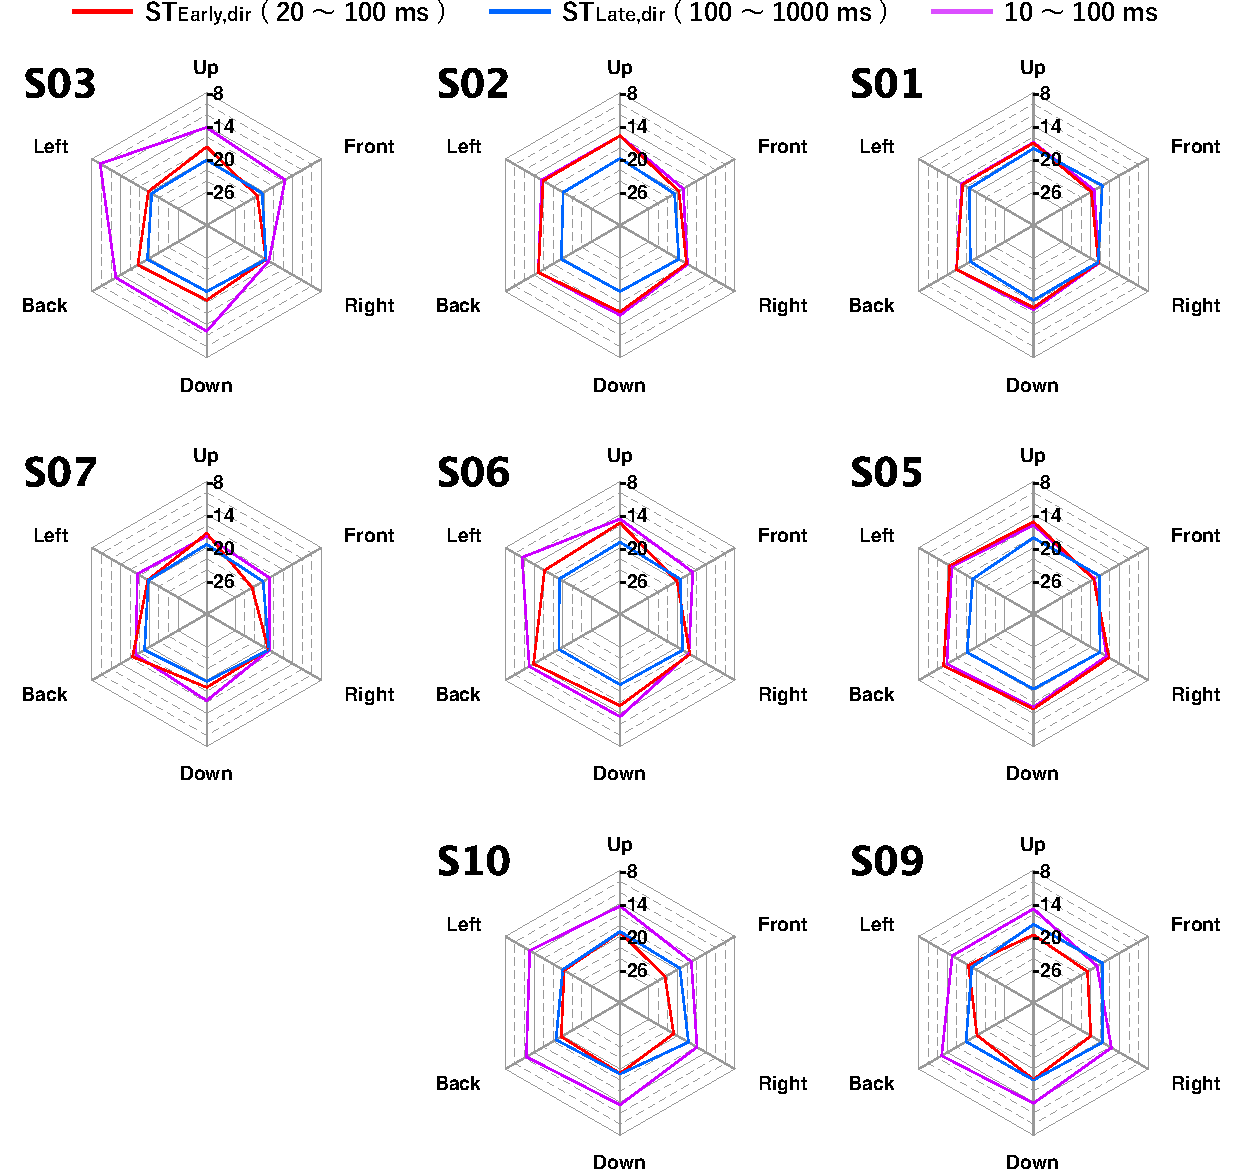
\includegraphics[scale=.75]{images/realHallDirSt/allPoint/reshaped/a.pdf}
  \caption{ホールA 方向別ST}
  \label{fig:ホールA 方向別ST}
\end{figure}

%=====================================================================
% ホールB
\newpage
\begin{figure}[H]
  \begin{minipage}{.5\linewidth} % 右側の図
    \centering
    \includegraphics[width=.7\linewidth]{images/measuredHalls/resized/picture_b.jpg}
    \\ホールB 外観
  \end{minipage}%
  \begin{minipage}{.5\linewidth} % 右側の図
    \centering
    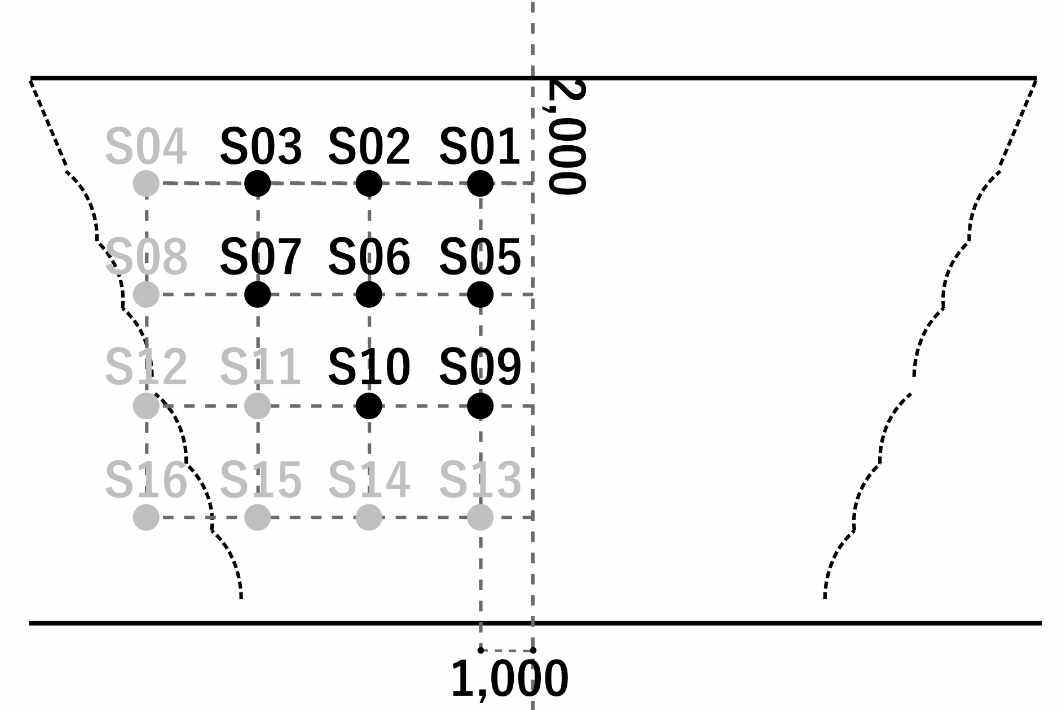
\includegraphics[width=.7\linewidth]{images/measuredHalls/resized/flat_b.jpg}
    \\ホールB 測定位置
  \end{minipage}

  \begin{minipage}{1\linewidth}
    \centering
    ホールB 諸元\\
    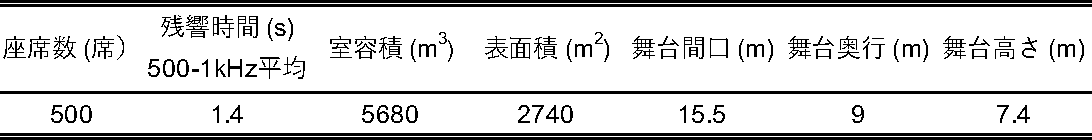
\includegraphics[width=.8\linewidth]{images/measuredHalls/informationTable/b.pdf}
  \end{minipage}
\end{figure}

\begin{figure}[H]
  \centering
  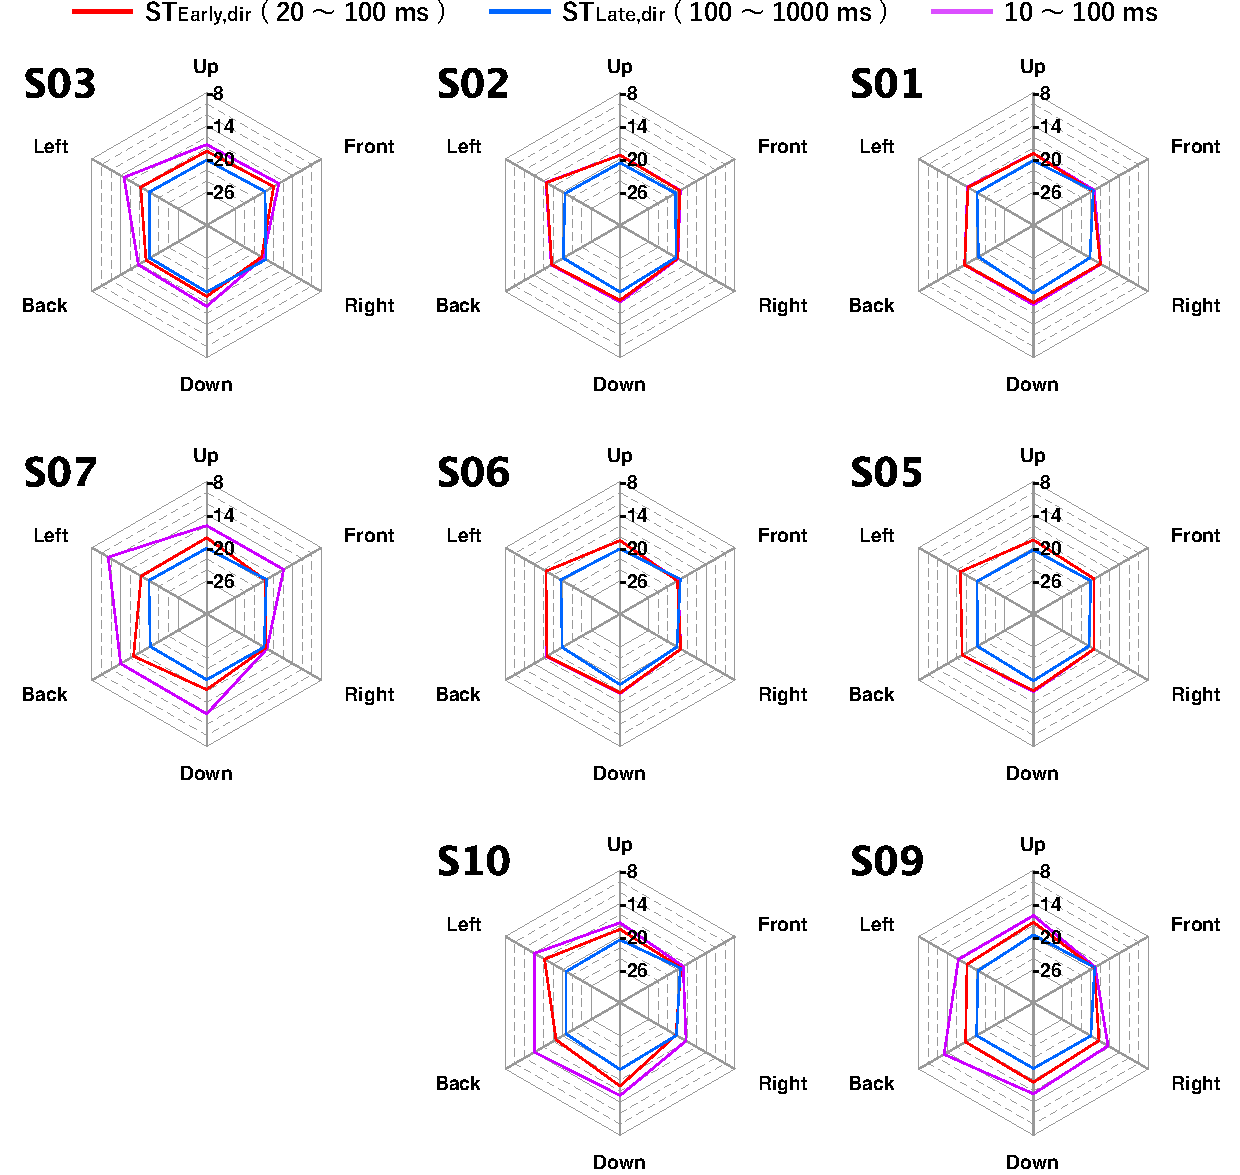
\includegraphics[scale=.75]{images/realHallDirSt/allPoint/reshaped/b.pdf}
  \caption{ホールB 方向別ST}
  \label{fig:ホールB 方向別ST}
\end{figure}

%=====================================================================
% ホールC
\newpage
\vspace*{6\baselineskip}

\begin{figure}[H]
  \begin{minipage}{.5\linewidth}
    \centering
    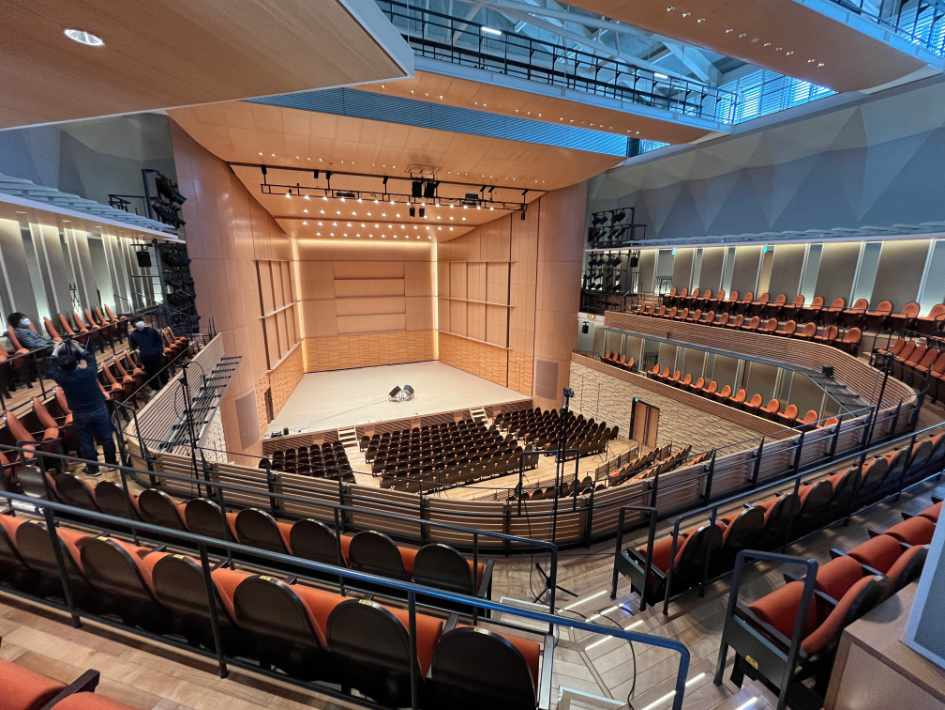
\includegraphics[width=.7\linewidth]{images/measuredHalls/resized/picture_c.jpg}
    \caption*{ホールC 外観}  
  \end{minipage}%
  \begin{minipage}{.5\linewidth}
    \centering
    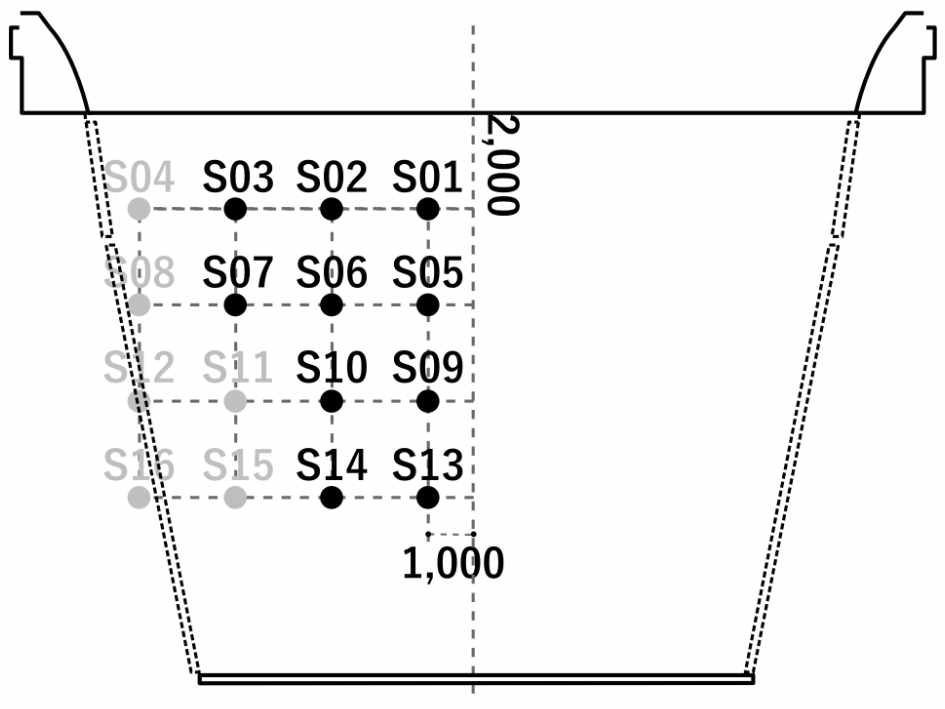
\includegraphics[width=.7\linewidth]{images/measuredHalls/resized/flat_c.jpg}
    \caption*{ホールC 測定位置}
  \end{minipage}
\end{figure}

\vspace{2\baselineskip}

\begin{table}[H]
  \centering
  \caption*{ホールC 諸元}
  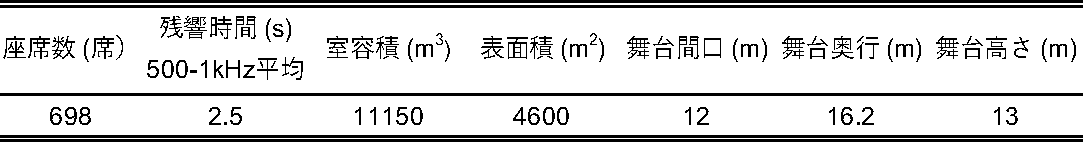
\includegraphics[width=.8\linewidth]{images/measuredHalls/informationTable/c_wide.pdf}
\end{table}

\newpage
\begin{figure}[H]
  \centering
  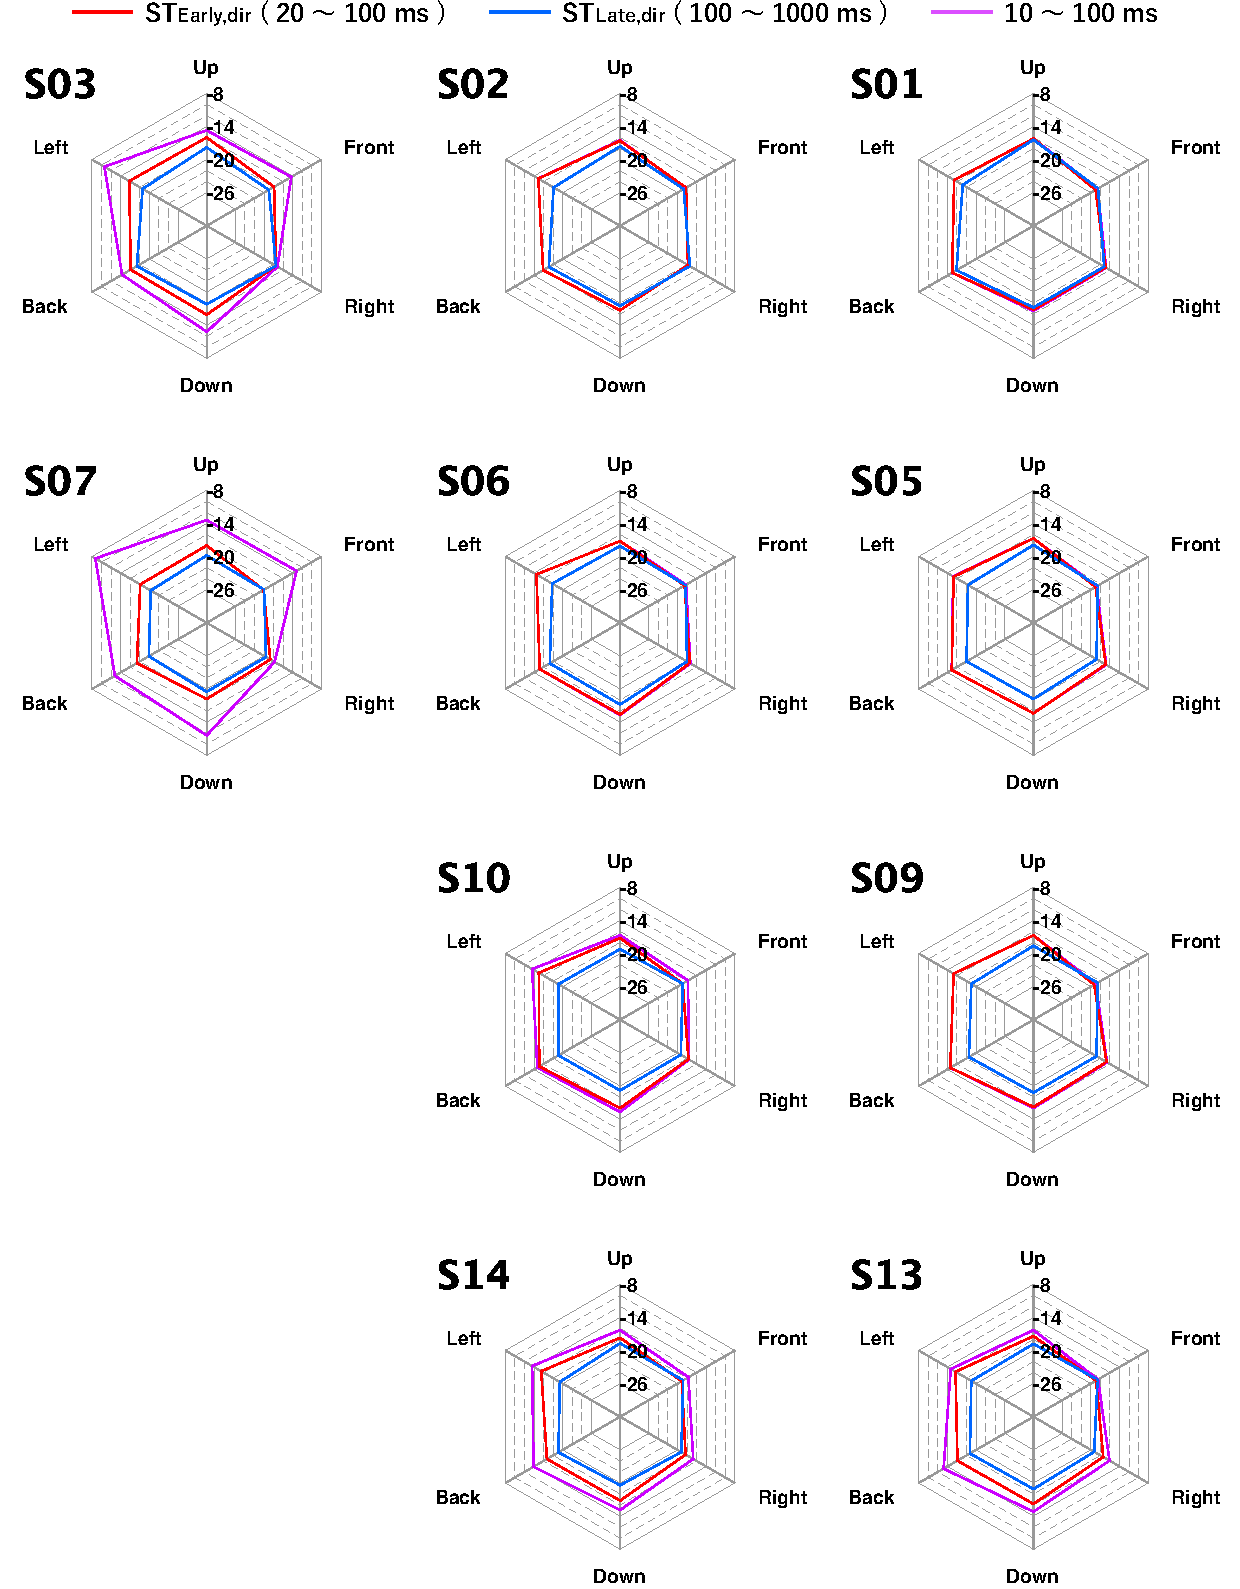
\includegraphics[scale=.75]{images/realHallDirSt/allPoint/reshaped/c.pdf}
  \caption{ホールC 方向別ST}
  \label{fig:ホールC 方向別ST}
\end{figure}

%=====================================================================
% ホールD
\newpage
\begin{figure}[H]
  \begin{minipage}{.5\linewidth} % 右側の図
    \centering
    \includegraphics[width=.7\linewidth]{images/measuredHalls/resized/picture_d.jpg}
    \\ホールD 外観
  \end{minipage}%
  \begin{minipage}{.5\linewidth} % 右側の図
    \centering
    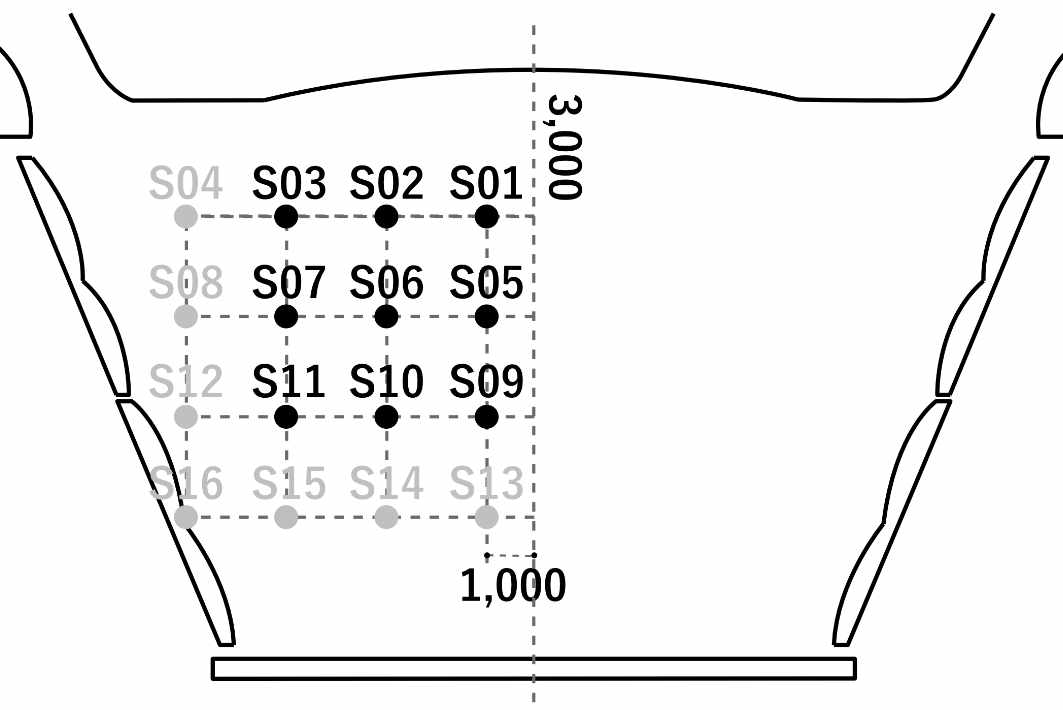
\includegraphics[width=.7\linewidth]{images/measuredHalls/resized/flat_d.jpg}
    \\ホールD 測定位置
  \end{minipage}

  \begin{minipage}{1\linewidth}
    \centering
    ホールD 諸元\\
    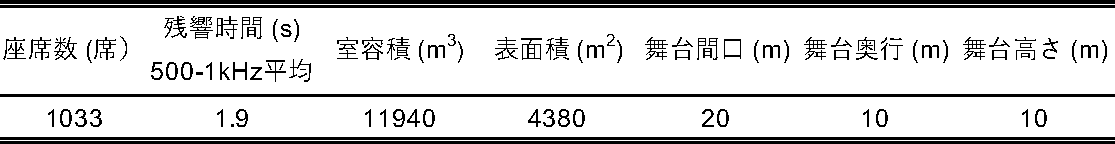
\includegraphics[width=.8\linewidth]{images/measuredHalls/informationTable/d.pdf}
  \end{minipage}
\end{figure}

\begin{figure}[H]
  \centering
  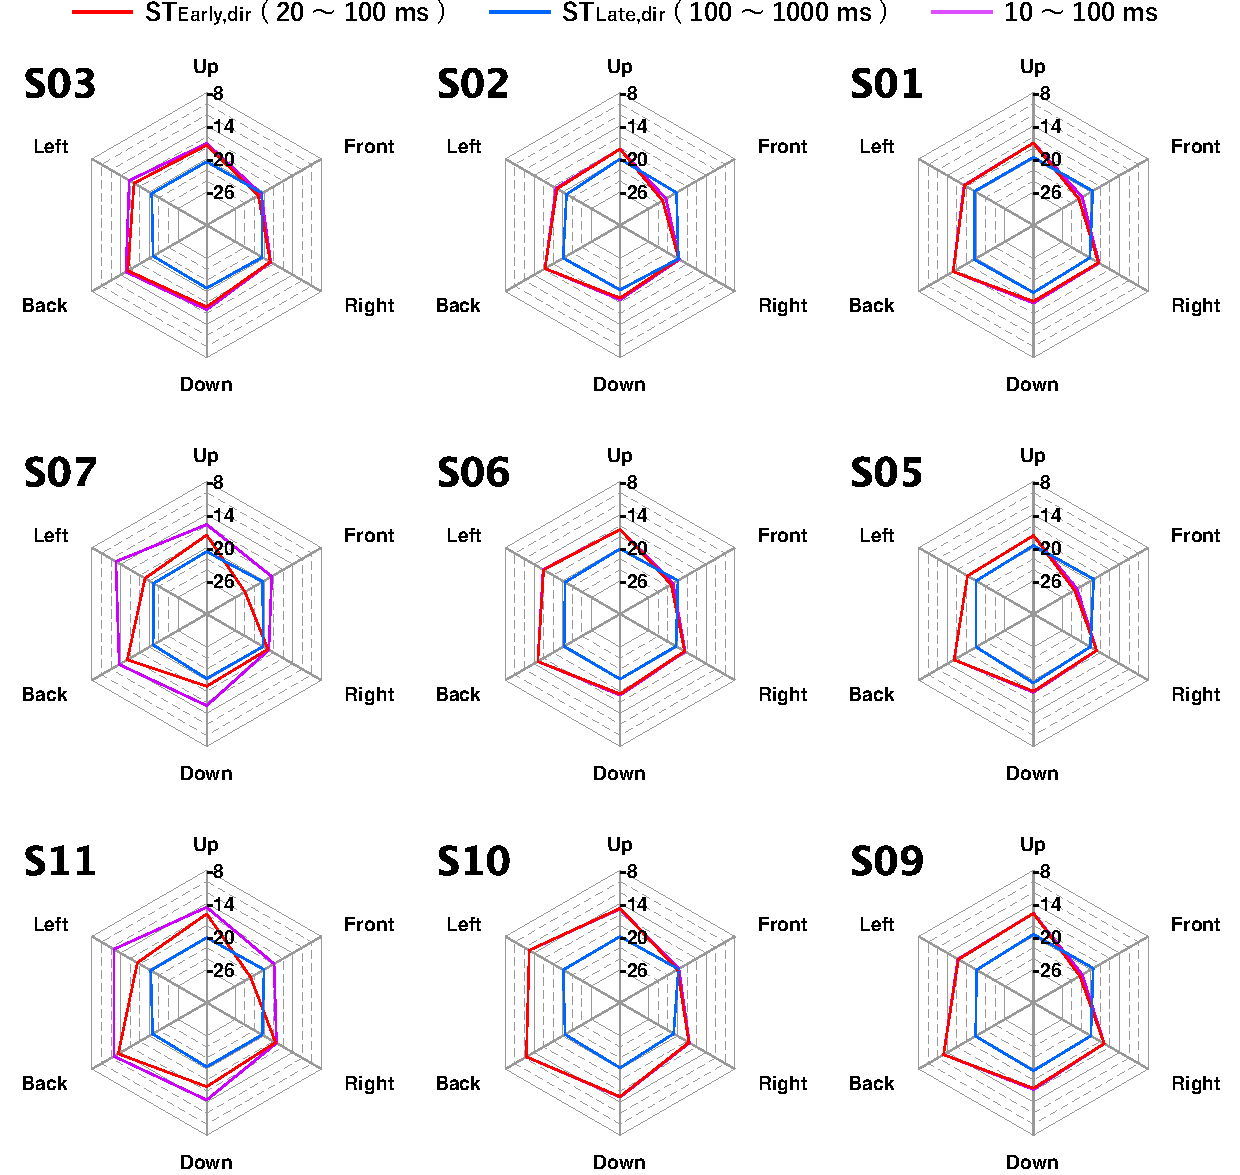
\includegraphics[scale=.77]{images/realHallDirSt/allPoint/reshaped/d.pdf}
  \caption{ホールD 方向別ST}
  \label{fig:ホールD 方向別ST}
\end{figure}

%=====================================================================
% ホールE
\newpage
\begin{figure}[H]
  \begin{minipage}{.5\linewidth} % 右側の図
    \centering
    \includegraphics[width=.7\linewidth]{images/measuredHalls/resized/picture_e.jpg}
    \\ホールE 外観
  \end{minipage}%
  \begin{minipage}{.5\linewidth} % 右側の図
    \centering
    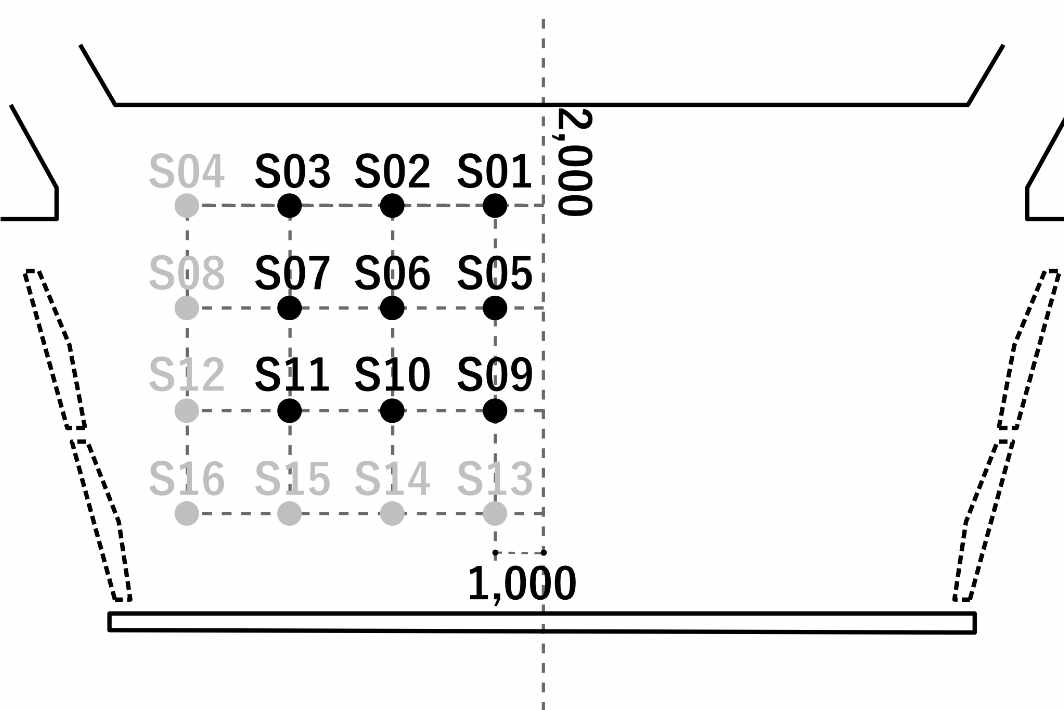
\includegraphics[width=.7\linewidth]{images/measuredHalls/resized/flat_e.jpg}
    \\ホールE 測定位置
  \end{minipage}

  \begin{minipage}{1\linewidth}
    \centering
    ホールE 諸元\\
    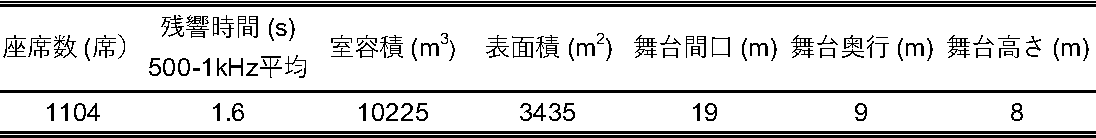
\includegraphics[width=.8\linewidth]{images/measuredHalls/informationTable/e.pdf}
  \end{minipage}
\end{figure}

\begin{figure}[H]
  \centering
  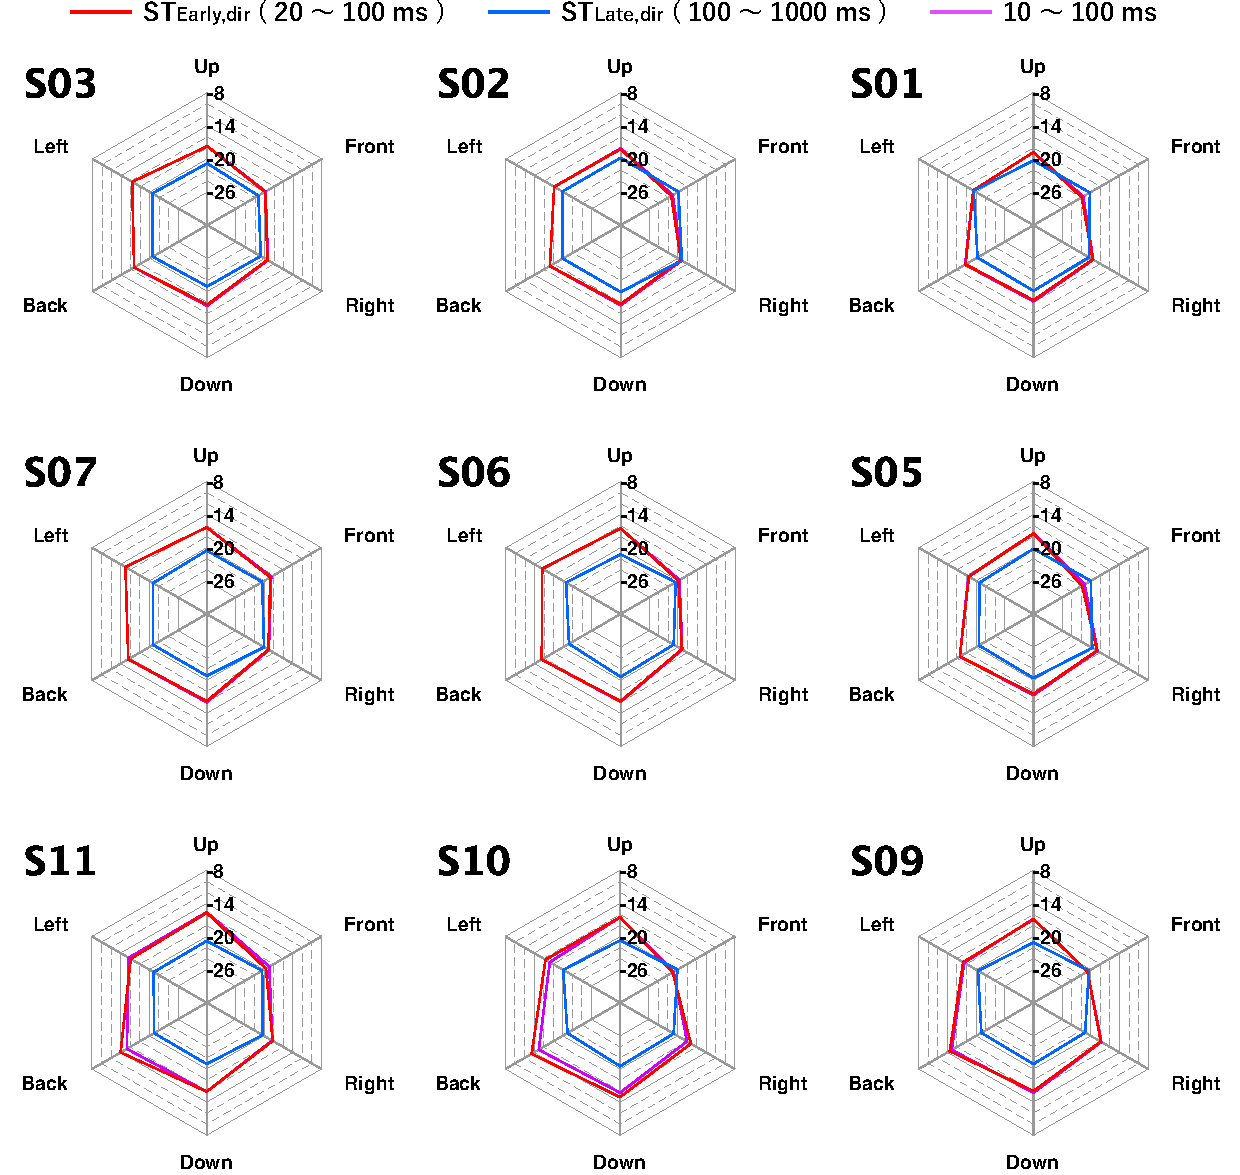
\includegraphics[scale=.77]{images/realHallDirSt/allPoint/reshaped/e.pdf}
  \caption{ホールE 方向別ST}
  \label{fig:ホールE 方向別ST}
\end{figure}

%=====================================================================
\newpage
\vspace{4\baselineskip}

\begin{figure}[H]
  \begin{minipage}{0.5\textwidth} % 左側の図
    \centering
    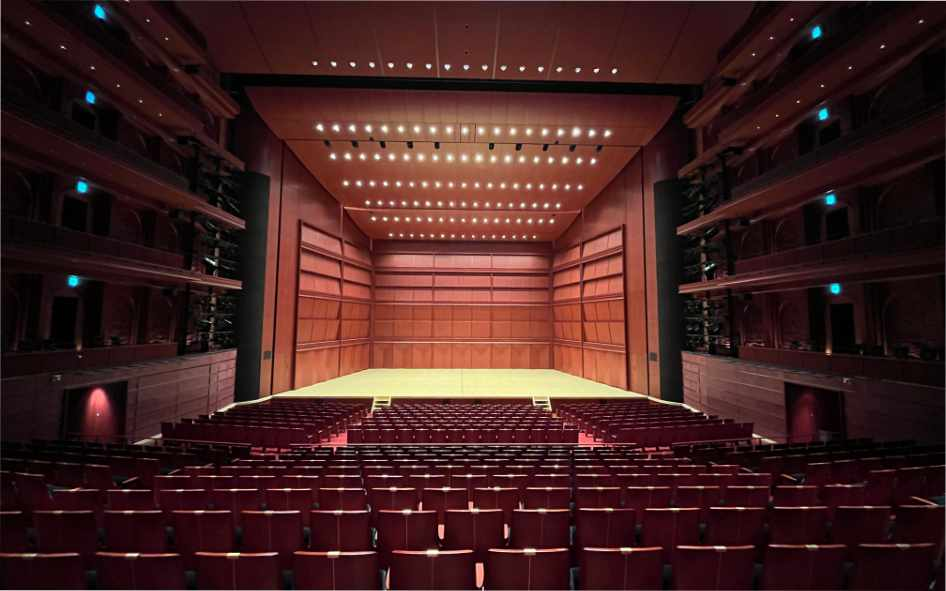
\includegraphics[width=.8\linewidth]{images/measuredHalls/resized/picture_f.jpg}
    \\ホールF 外観
    \vspace{2\baselineskip}

    ホールF 諸元\\
    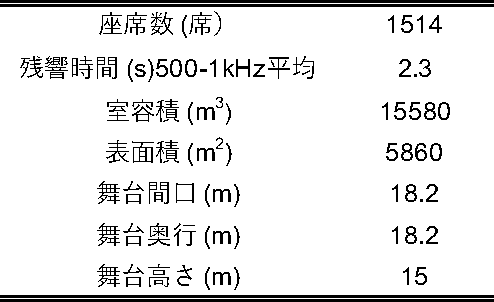
\includegraphics[width=.8\linewidth]{images/measuredHalls/informationTable/f.pdf}
    \vspace{2\baselineskip}

    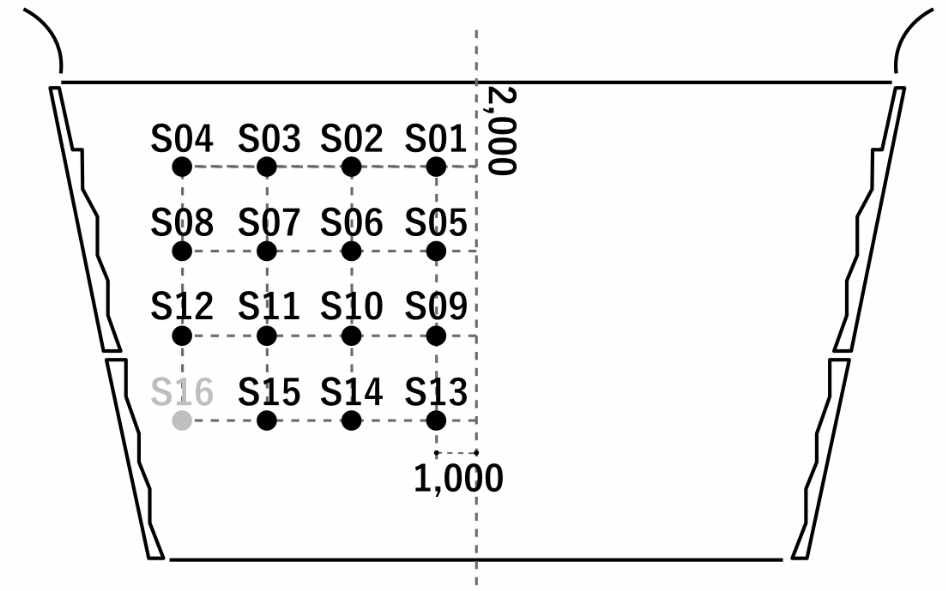
\includegraphics[width=.8\linewidth]{images/measuredHalls/resized/flat_f.jpg}
    \\ホールF 測定位置
  \end{minipage}%
  \begin{minipage}{.5\linewidth} % 右側の図
    \raggedleft
    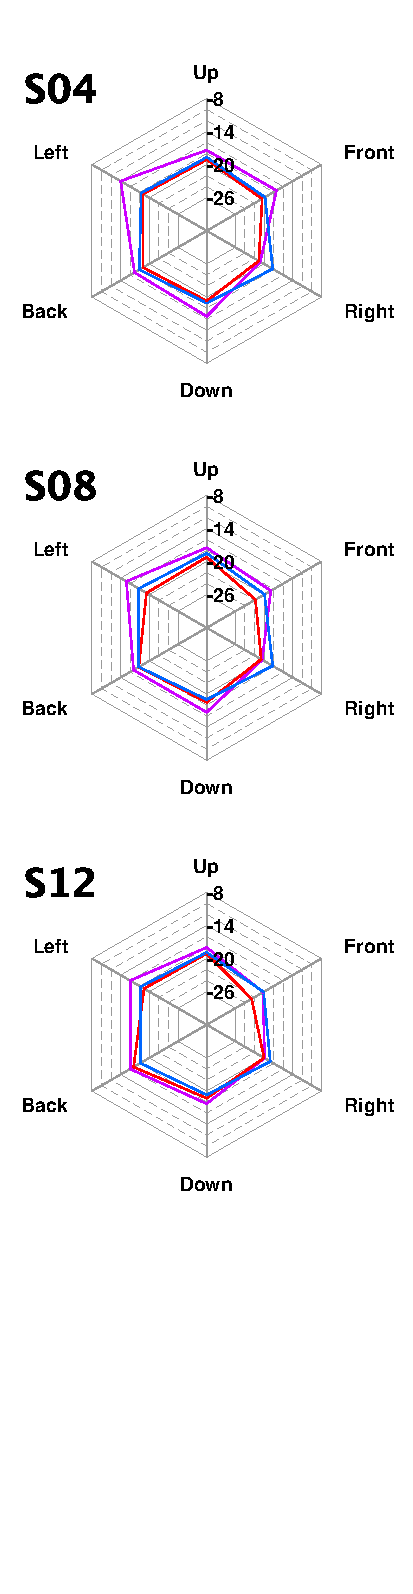
\includegraphics[scale=.77]{images/realHallDirSt/allPoint/reshaped/fLeftPage.pdf}
  \end{minipage}
\end{figure}

\newpage

\begin{figure}[H]
  \centering
  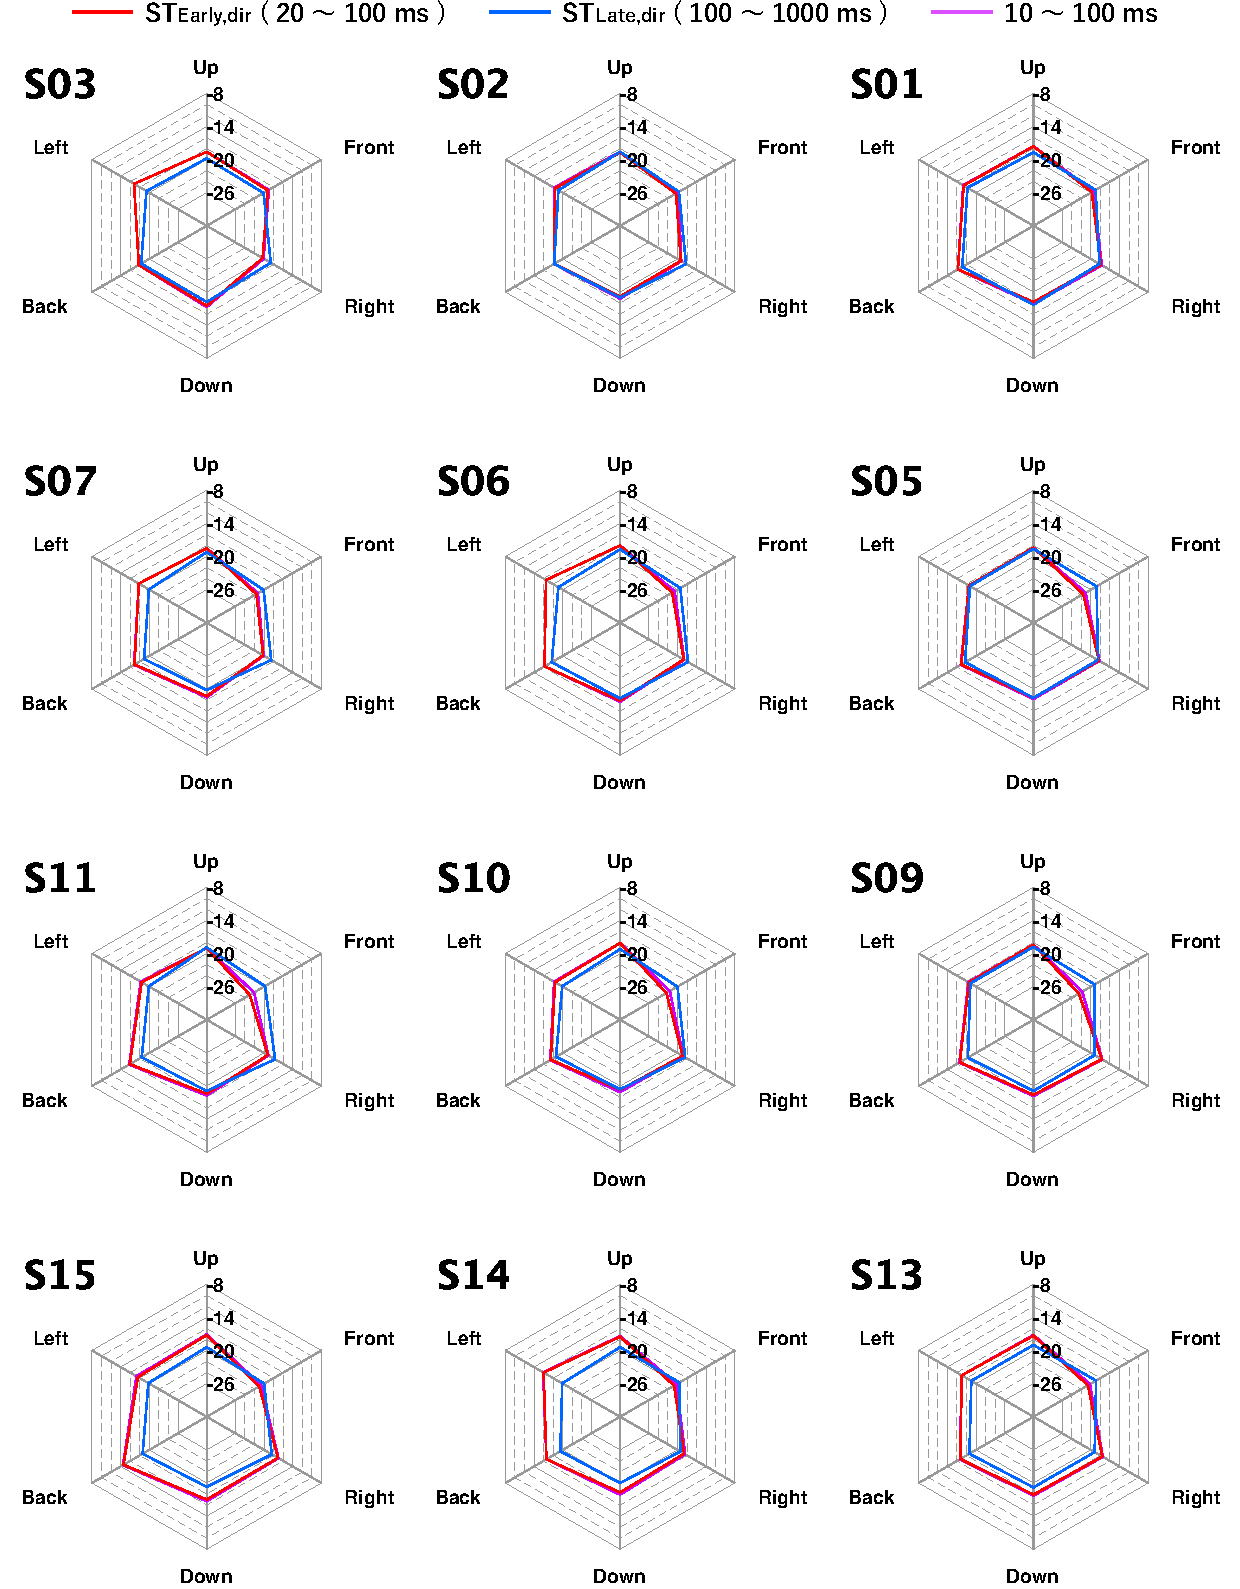
\includegraphics[scale=.77]{images/realHallDirSt/allPoint/reshaped/fRightPage.pdf}
  \caption{ホールF 方向別ST}
  \label{fig:ホールF 方向別ST}
\end{figure}

%=======================================================================
\newpage
  
\vspace{4\baselineskip}

\begin{figure}[H]
  \begin{minipage}{0.5\textwidth} % 左側の図
    \centering

    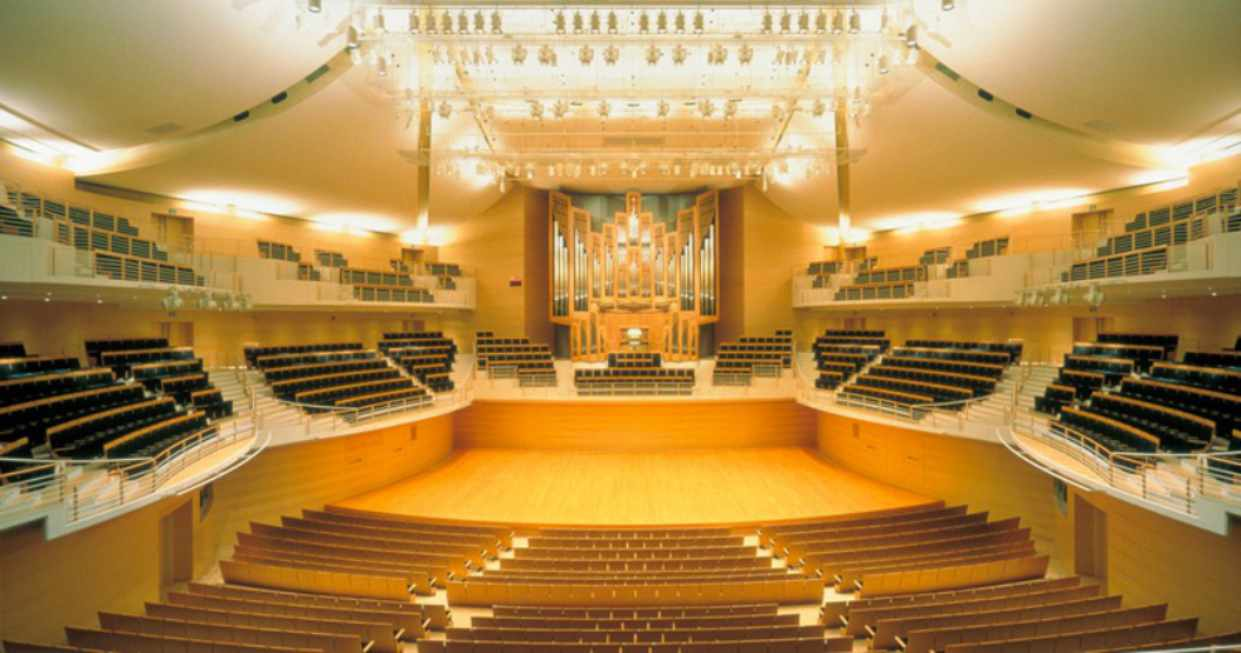
\includegraphics[width=.8\linewidth]{images/measuredHalls/resized/picture_g.jpg}
    \\ホールG 外観
    \vspace{2\baselineskip}

    ホールG 諸元\\
    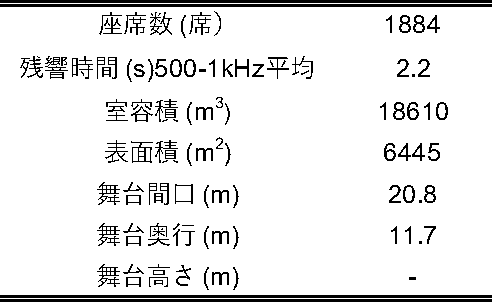
\includegraphics[width=.8\linewidth]{images/measuredHalls/informationTable/g.pdf}
    \vspace{2\baselineskip}

    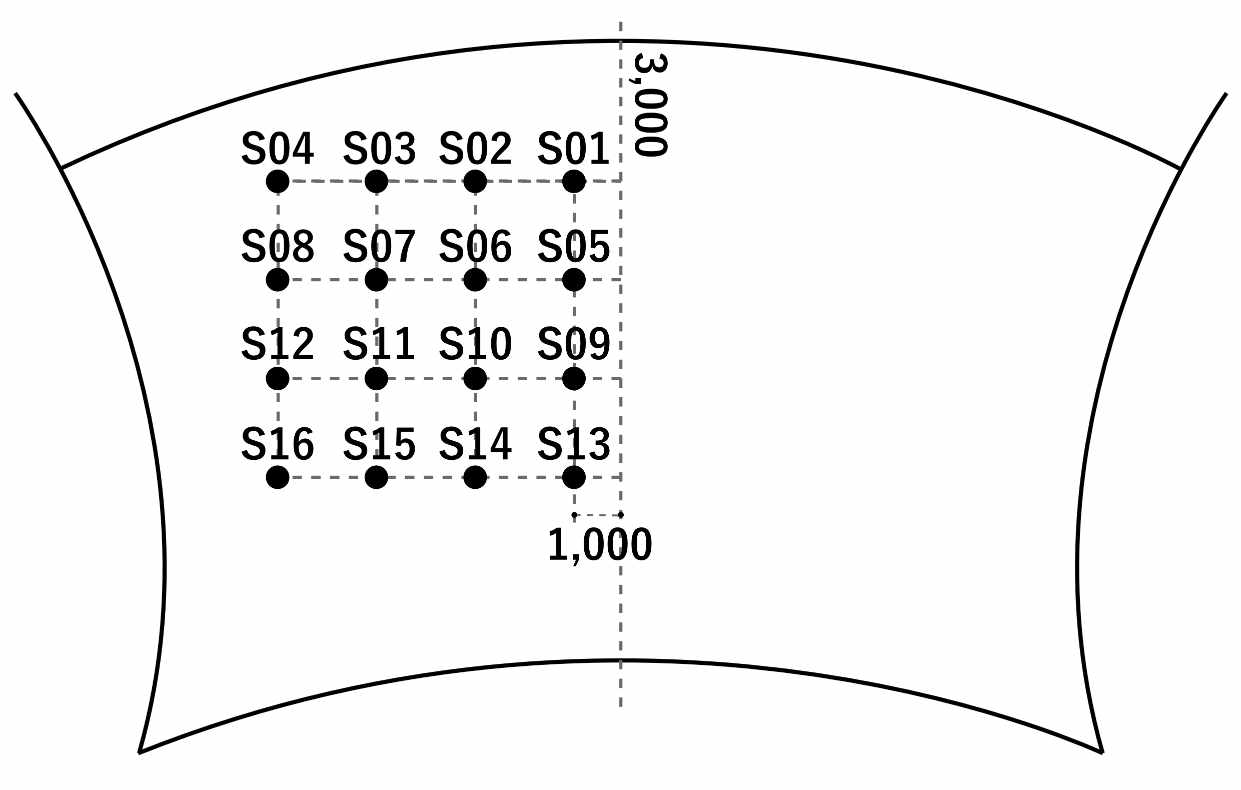
\includegraphics[width=.8\linewidth]{images/measuredHalls/resized/flat_g.jpg}
    \\ホールG 測定位置
  \end{minipage}%
  \begin{minipage}{.5\linewidth} % 右側の図
    \raggedleft
    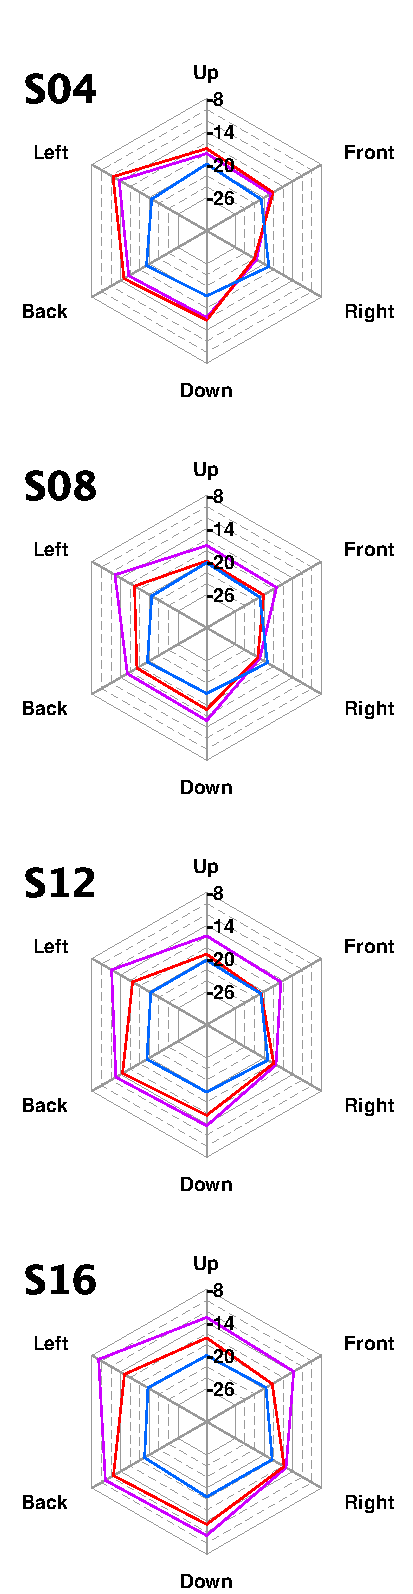
\includegraphics[scale=.77]{images/realHallDirSt/allPoint/reshaped/gLeftPage.pdf}
  \end{minipage}
\end{figure}

\newpage

\begin{figure}[H]
  \centering
  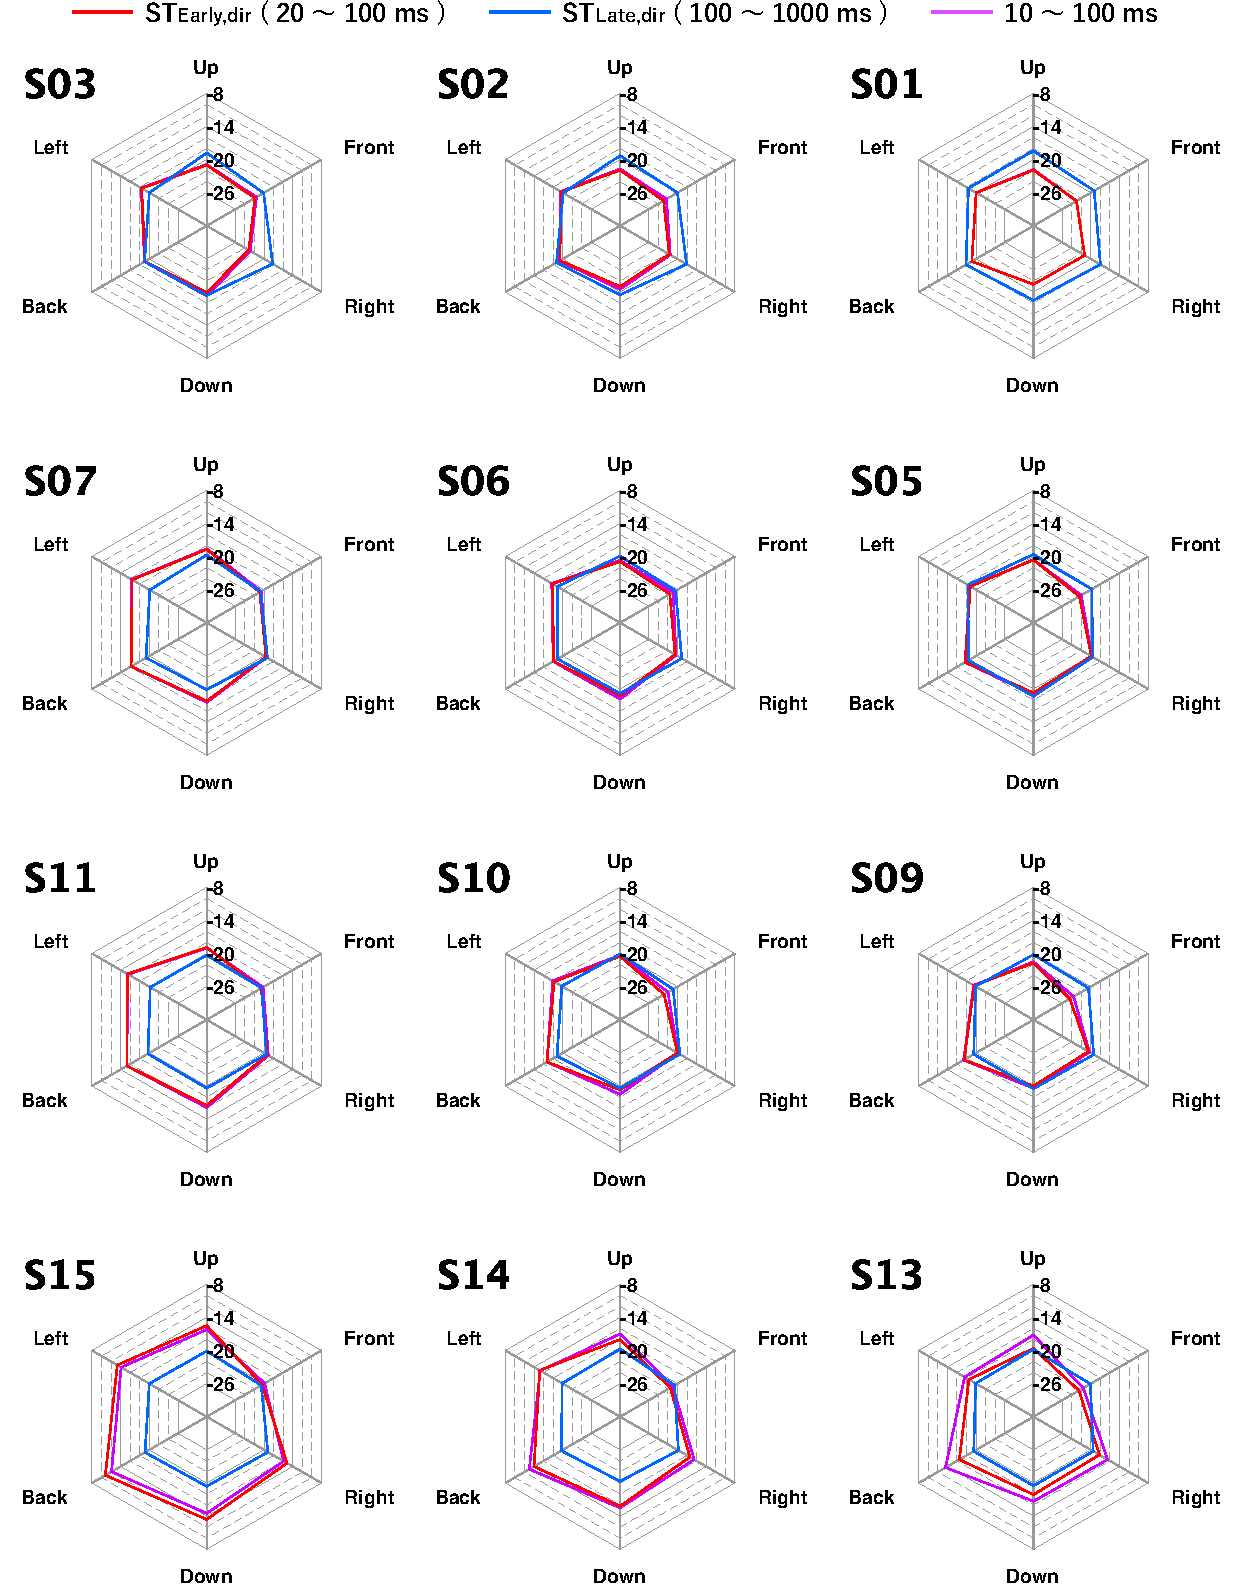
\includegraphics[scale=.77]{images/realHallDirSt/allPoint/reshaped/gRightPage.pdf}
  \caption{ホールG 方向別ST}
  \label{fig:ホールG 方向別ST}
\end{figure}

\clearpage

%=======================================================================
\subsection*{測定結果の考察}

前項にて、各ホールの全測定点における$\mathrm{ST_{Early,dir}}$、$\mathrm{ST_{Early,dir}}$および$10$~$\SI{100}{\ms}$での方向別反射音のエネルギーの評価値について、測定結果を示した。

さらに、$\mathrm{ST_{Early,dir}}$および$\mathrm{ST_{Early,dir}}$のホール間での傾向の違いについて、各ホールにおけるすべての測定点の平均値と最大値・最小値を図\ref{fig:各ホールのSTEarlyの平均値と最大値・最小値}および図\ref{fig:各ホールのSTLateの平均値と最大値・最小値}に示し、また$\mathrm{ST_{Early,dir}}$および$\mathrm{ST_{Early,dir}}$の測定位置による傾向の違いについて、各測定位置におけるすべてのホールでの平均値と最大値・最小値を図\ref{fig:各ホールのSTEarlyの平均値と最大値・最小値}および図\ref{fig:各ホールのSTLateの平均値と最大値・最小値}に示す。ただし、\ref{fig:各ホールのSTEarlyの平均値と最大値・最小値}および図\ref{fig:各ホールのSTLateの平均値と最大値・最小値}では、すべてのホールで測定を行った測定点であるS01、S02、S03、S05、S06、S07、S09、S10の結果について計算した。

\subsubsection{初期反射音に関する評価について}

$\mathrm{ST_{Early,dir}}$および$10$~$\SI{100}{\ms}$に到来する反射音については、全ホールに共通して方向別の偏差が見られ、方向ごとに強度が異なっていた。特に、すべての測定位置でFrontの値が相対的に低く、$\SI{100}{\ms}$までに到来する客席側からの反射音レベルが低くなっている傾向が見られた。

舞台中央側および前方側の測定点では$\mathrm{ST_{Early,dir}}$と$10$~$\SI{100}{\ms}$に到来する反射音の評価値はほぼ等しいのに対し、壁面との距離の近い舞台上手側および舞台奥付近の測定点では、特にLeftおよびBackの方向で$10$~$\SI{100}{\ms}$の評価値が$\mathrm{ST_{Early,dir}}$よりも顕著に大きくなる傾向が見られた。$\SI{100}{\ms}$以内に到来する反射に占める一次の反射音のエネルギーが大きく、これが評価区間に含まれるかどうかによって評価値が大きく変化していると考えられる。また、壁面の近傍における測定点ではこの一次の反射音の減衰も小さく、$10$~$\SI{20}{\ms}$に到来している成分のエネルギーが特に大きくなっていると考えられる。ごく短い遅れ時間で到来する反射音はカラレーションを引き起こす恐れがあり、$10$~$\SI{20}{\ms}$の間に到来する反射音もカラレーションを起こして心理印象を変化させる原因になりうるため、これらの点におけるエネルギー量に着目した指標での評価は心理印象とうまく対応しない可能性がある。


\subsubsection{後期反射音に関する評価について}
$\mathrm{ST_{Late,dir}}$については、方向別の差異が小さい傾向にあり、$100$~$\SI{1000}{\ms}$に到来する反射音は一様な強度になっていて、拡散してあらゆる方向から到来していると考えられる。また、同一のホール内での測定点毎の差も小さく、舞台上での位置依存性も小さいと推察される。一方で、ホール間での差異は大きい傾向にあり、ホールCおよびFは他のホールに比べて全体的に値が高くなっている。ホールCおよびFは残響時間も$\SI{2}{秒}$以上とホールA、B、D、Eに比べてかなり長くなっているが、同じく$\SI{2}{秒}$以上の長い残響時間を有すホールGにおける$\mathrm{ST_{Late,dir}}$は他のホールと同程度の水準である。ホールAからFがシューボックス型の形状をしているのに対し、ホールGはアリーナ型の形状であるため、ホールGでは残響時間の長さの割に演奏者に返る後期反射音が少なく、$\mathrm{ST_{Late,dir}}$がホールC、Fよりも小さくなっているのではないかと考えられる。
%=======================================================================

\newpage
\vspace*{\stretch{1}}
\begin{figure}[H]
  \centering
  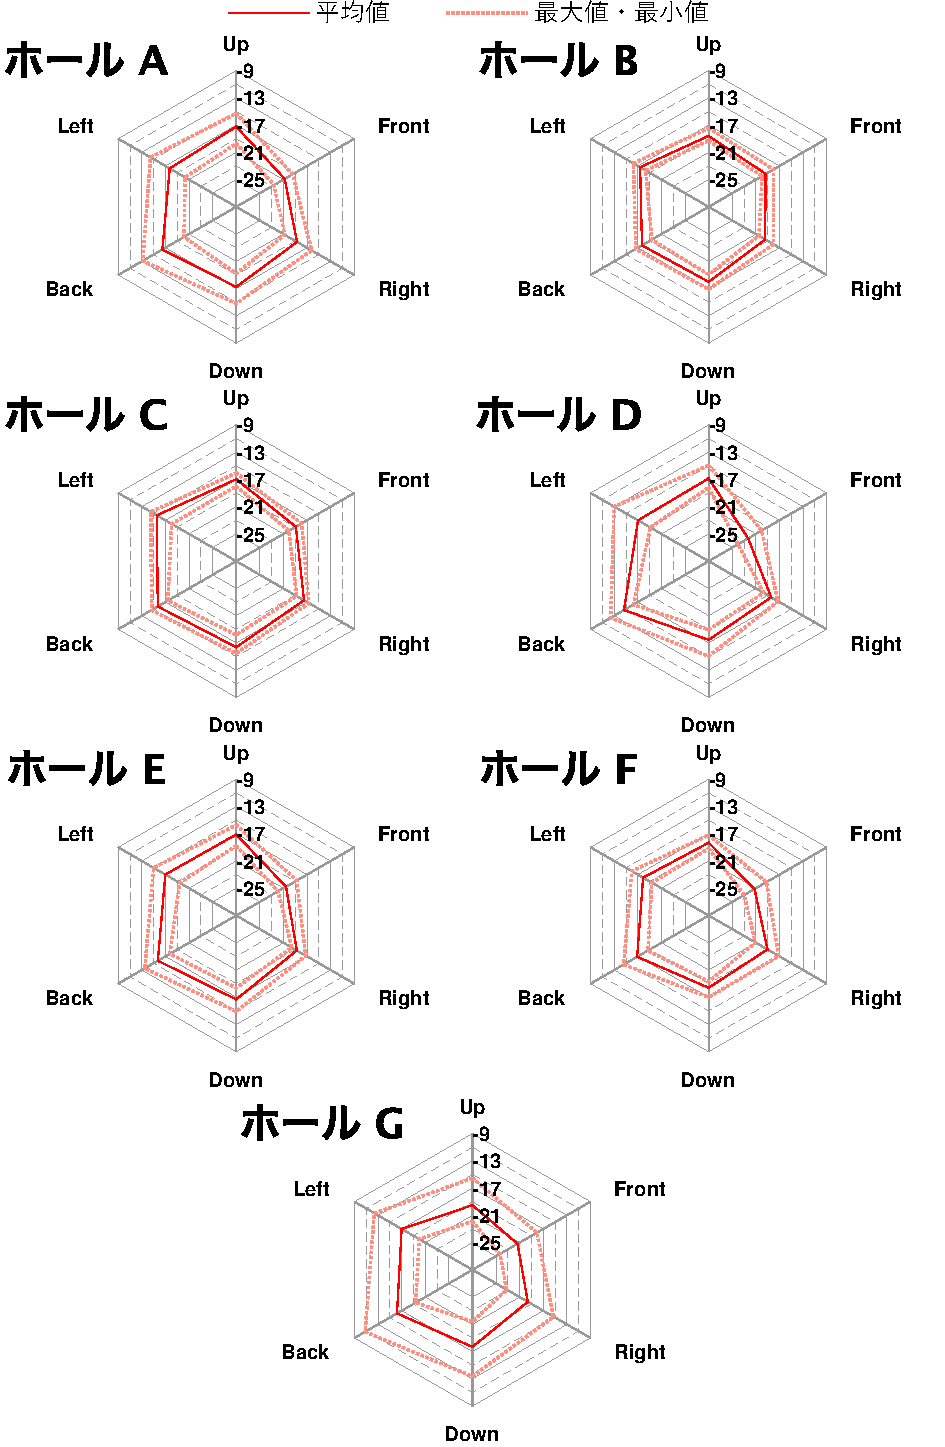
\includegraphics[scale=.8]{images/realHallDirSt/realHallOverall/eachHallEarly.pdf}
  \caption{各ホールの$\mathrm{ST_{Early,dir}}$の平均値と最大値・最小値}
  \label{fig:各ホールのSTEarlyの平均値と最大値・最小値}
\end{figure}
\vspace*{\stretch{1}}

%=======================================================================

\newpage
\vspace*{\stretch{1}}
\begin{figure}[H]
  \centering
  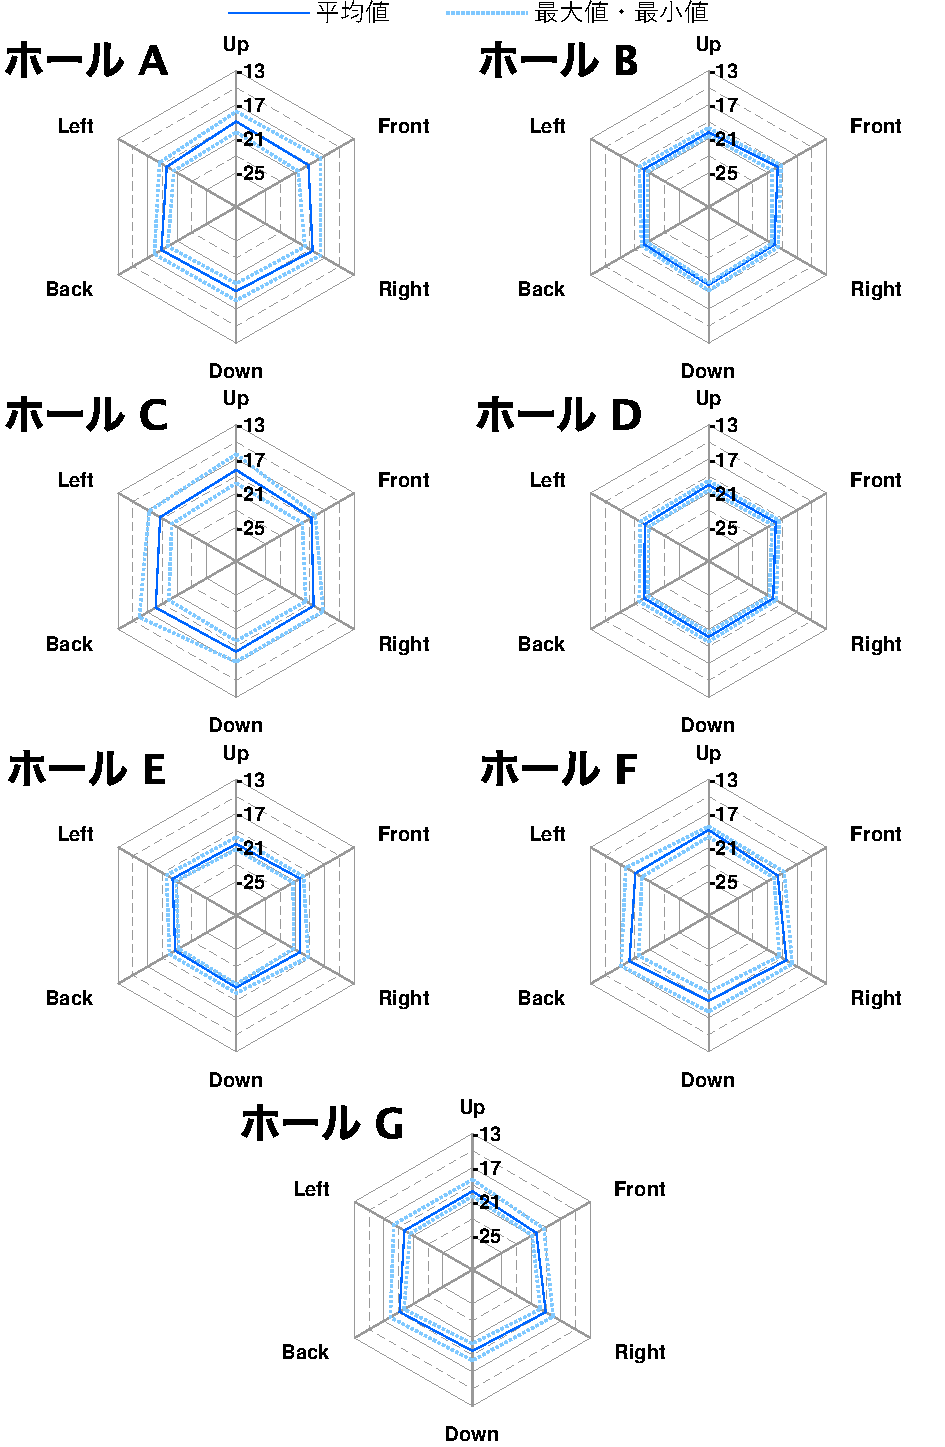
\includegraphics[scale=.8]{images/realHallDirSt/realHallOverall/eachHallLate.pdf}
  \caption{各ホールの$\mathrm{ST_{Late,dir}}$の平均値と最大値・最小値}
  \label{fig:各ホールのSTLateの平均値と最大値・最小値}
\end{figure}
\vspace*{\stretch{1}}

%=======================================================================

\newpage
\vspace*{\stretch{1}}
\begin{figure}[htbp]
  \centering
  \includegraphics[scale=.8]{images/realHallDirSt/realHallOverall/eachPointEarly.pdf}
  \caption{各測定点の$\mathrm{ST_{Early,dir}}$の平均値と最大値・最小値}
  \label{fig:各測定位置のSTEarlyの平均値と最大値・最小値}
\end{figure}
\vspace*{\stretch{1}}

%=======================================================================

\newpage
\vspace*{\stretch{1}}
\begin{figure}[htbp]
  \centering
  \includegraphics[scale=.8]{images/realHallDirSt/realHallOverall/eachPointLate.pdf}
  \caption{各測定点の$\mathrm{ST_{Late,dir}}$の平均値と最大値・最小値}
  \label{fig:各測定位置のSTLateの平均値と最大値・最小値}
\end{figure}
\vspace*{\stretch{1}}
%=======================================================================

\newpage
\section{生成音場の目標値の設定}
方向特性の評価を行う演奏実験を行う音場について、実際のコンサートホールのステージ上の音場に近づけることを目指して生成を試みる。壁面に近い測定点での測定結果では、カラレーションの発生に大きく寄与しうる$10$~$\SI{20}{\ms}$のごく短い時間に到来する一次の反射音のエネルギーが大きく、エネルギーの値に着目して構築された指標値である$\mathrm{ST_{Early,dir}}$によって適切に音場が記述されない恐れがあるため、ステージ中央・前方付近の測定点であるS01,S02,S05,S06の4点の測定結果を用いて基準とする音場の目標値を設定する。これらの標準的な演奏位置とも対応し、現実の演奏条件を模倣する音場生成の目標値の設定として妥当であると考えられる。

まず、測定位置の違いとホールによる違いを平均化するため、測定を実施した7つすべてのホールでのこの4点での測定結果の平均値を算出した。さらに、測定を上手側反面で行なったことによる左右の偏りを補正するため、左右方向の値を平均して、基準とする音場の生成の目標値として設定した。これを図\ref{fig:生成音場の目標値}に示す。

\vspace{\stretch{1}}

\begin{figure}[H]
  \begin{minipage}[b]{.5\textwidth}
    \centering
    \includegraphics[width=.8\linewidth]{images/realHallDirSt/targetField/early.pdf}
  \end{minipage}%
  \begin{minipage}[b]{.5\textwidth}
    \centering
    \includegraphics[width=.8\linewidth]{images/realHallDirSt/targetField/late.pdf}
  \end{minipage}

  \caption{生成音場の目標値}
  \label{fig:生成音場の目標値}
\end{figure}

\vspace{\stretch{1}}

%=======================================================================


% 参考文献
% 参考文献の箇所にインプットしてください。

% 分割ファイル内でのみ,bibliographyを読み込みます。

\expandafter\ifx\csname ifdraft\endcsname\relax

  % bibliographyを展開する

  \bibliographystyle{junsrt}
  \bibliography{ref.bib}% 同じディレクトリ内のbibファイルのみを参照可能

\fi

\end{document}